% Biên dịch trên Overleaf: Compiler = pdfLaTeX. Upload cả thư mục report/.
\documentclass[conference]{IEEEtran}
\usepackage[T5]{fontenc}
\usepackage[utf8]{inputenc}
\usepackage[vietnamese]{babel}
\usepackage{amsmath,amssymb,amsthm}
\usepackage{graphicx}
\usepackage{booktabs}
\usepackage{algorithm}
\usepackage{algpseudocode}
\usepackage{cite}
\usepackage{url}
\graphicspath{{figures/}}
\newtheorem{theorem}{Định lý}
\newtheorem{lemma}{Bổ đề}

\begin{document}

\title{LogiGraph: Tối ưu hóa mạng lưới giao hàng và định tuyến vận tải đô thị\\
trên dữ liệu bản đồ thực tế nội thành Hà Nội}

\author{\IEEEauthorblockN{TV1 \quad TV2 \quad TV3 \quad TV4 \quad TV5}
\IEEEauthorblockA{Học phần Cấu trúc dữ liệu và Giải thuật nâng cao\\
Khoa Công nghệ Thông tin, Trường Đại học Công nghệ Kỹ thuật Hưng Yên}}

\maketitle

\begin{abstract}
Bài báo trình bày LogiGraph, hệ thống định tuyến giao hàng và quy hoạch mạng lưới kho trên dữ liệu bản đồ thật của 24 phường
nội thành Hà Nội lấy từ OpenStreetMap (38\,604 đỉnh, 69\,411 cạnh có hướng). Toàn bộ cấu trúc dữ liệu lõi được tự cài đặt
chỉ bằng mảng, không dùng bảng băm hay hàng đợi dựng sẵn: đồ thị có trọng số biểu diễn bằng Adjacency List; hàng đợi ưu tiên
thích ứng có Locator phục vụ Dijkstra và tính lại tuyến khi có tắc hoặc cấm đường; Union-Find với union by rank và path
compression phục vụ Kruskal, kiểm tra liên thông và phân cụm giao hàng; quy hoạch động cho bài toán xếp hàng 0/1 Knapsack và
TSP bất đối xứng (Held-Karp). Mỗi giải thuật được kiểm tra chéo với một lời giải chuẩn bằng 81 test tự động. Thực nghiệm trên
đồ thị tới 50\,000 đỉnh cho thấy: Union-Find giữ khoảng 1{,}2 bước mỗi thao tác từ $10^3$ đến $10^6$ phần tử; Bellman-Ford
và Dijkstra dùng mảng chậm hơn Dijkstra dùng heap từ 13 tới hơn 146 lần; và lợi thế của hàng đợi thích ứng so với heap lazy
phụ thuộc mật độ đồ thị, rõ rệt trên đồ thị dày nhưng không xuất hiện trên mạng đường gần phẳng. Quy tắc bỏ qua sự cố nằm ngoài
tuyến giúp phản hồi trong 0{,}4 ms thay vì khoảng 110 ms khi phải tính lại.
\end{abstract}

\begin{IEEEkeywords}
Dijkstra, Adaptable Priority Queue, Union-Find, Kruskal, Knapsack, Held-Karp, định tuyến đô thị, OpenStreetMap
\end{IEEEkeywords}

\section{Giới thiệu}\label{sec:intro}

Giao hàng chặng cuối trong đô thị gồm nhiều bài toán con chạy trên cùng một mạng đường: tìm tuyến đi nhanh nhất giữa hai điểm, tính lại tuyến khi một đoạn đường bị tắc hoặc bị cấm, quy hoạch mạng tuyến nối các kho trung chuyển với chi phí nhỏ nhất, chọn kiện hàng lên xe theo tải trọng và sắp thứ tự các điểm giao. Mỗi bài toán con ứng với một cấu trúc dữ liệu hoặc giải thuật kinh điển: Dijkstra với hàng đợi ưu tiên~\cite{dijkstra1959,goodrich2013}, cây khung nhỏ nhất với Union-Find~\cite{kruskal1956,tarjan1975}, và quy hoạch động cho Knapsack và TSP~\cite{bellman1958,heldkarp1962}. Khó khăn khi đưa các giải thuật này vào một hệ thống là chúng phải dùng chung một biểu diễn đồ thị, chung một dữ liệu, và kết quả của bước này là đầu vào của bước sau.

LogiGraph là đồ án nhóm của học phần Cấu trúc dữ liệu và Giải thuật nâng cao (Đề tài~4). Hệ thống cài đặt lại từ đầu các cấu trúc trên bằng Python thuần, chạy trên mạng đường ô tô nội thành Hà Nội lấy từ OpenStreetMap~\cite{osm} với 38.604 Intersection và 69.411 Road Segment, và có một ứng dụng web để trình diễn trực tiếp. Trong báo cáo, \emph{Intersection} là một đỉnh của đồ thị, \emph{Road Segment} là một cạnh có hướng, \emph{Travel Time} là trọng số tính bằng giây, \emph{Hub} là kho trung chuyển đặt tại một Intersection, \emph{Parcel} là kiện hàng và \emph{Trip} là một chuyến xe xuất phát và quay về một Hub.

\subsection{Yêu cầu bài toán}

Đề tài đặt ra năm yêu cầu chức năng:
\begin{enumerate}
\item[(R1)] Mô hình hóa mạng đường bằng đồ thị có hướng, có trọng số: đỉnh là giao lộ hoặc kho, cạnh là đoạn đường với trọng số quãng đường hoặc thời gian.
\item[(R2)] Tìm đường ngắn nhất, cho phép cập nhật trọng số động (tắc đường, cấm đường) và tính lại tuyến ngay.
\item[(R3)] Xây mạng xương sống chi phí nhỏ nhất giữa các Hub bằng Union-Find và Kruskal.
\item[(R4)] Chọn kiện lên xe bằng 0/1 Knapsack và sắp thứ tự giao bằng TSP quy mô nhỏ, cả hai giải bằng quy hoạch động.
\item[(R5)] Kiểm tra tính liên thông và phân vùng giao hàng theo đơn vị hành chính.
\end{enumerate}
Kèm theo là hai ràng buộc: các cấu trúc lõi phải tự cài đặt, không dùng \texttt{dict}/\texttt{set} dựng sẵn để thay thế; và phải có benchmark trên bản đồ thật từ 10.000 đỉnh trở lên, so sánh với các baseline cơ bản. Bảng~\ref{tab:req} ánh xạ từng yêu cầu tới cấu trúc dữ liệu, module và thành viên phụ trách.

Có hai điểm chúng tôi làm khác với câu chữ của đề và nêu rõ ở đây. Thứ nhất, từ ngày 01/07/2025 Việt Nam bỏ cấp quận/huyện, nên trên OpenStreetMap ranh giới \texttt{admin\_level=6} tại Hà Nội nay là các phường mới. Hệ thống vì vậy phân vùng theo 24 phường giao với vùng bản đồ đã chọn thay cho quận (Mục~\ref{sec:graph}). Thứ hai, đồ thị Hub là đồ thị đầy đủ nên về lý thuyết Prim cài bằng mảng ($O(H^2)$) phù hợp hơn Kruskal ($O(H^2\log H)$). Chúng tôi vẫn dùng Kruskal với Union-Find như đề yêu cầu, vì thực nghiệm cho thấy ở quy mô vài trăm Hub, Kruskal nhanh hơn khoảng hai lần (Mục~\ref{sec:experiments}); Prim mảng được giữ làm lời giải đối chiếu trong test. Kruskal còn được dùng cho phân cụm single-linkage~\cite{gower1969} (Mục~IV).

\begin{table*}[t]
\centering
\caption{Ánh xạ yêu cầu chức năng tới cấu trúc dữ liệu, module và thành viên phụ trách}
\label{tab:req}
\begin{tabular}{@{}p{0.20\textwidth}p{0.40\textwidth}p{0.22\textwidth}c@{}}
\toprule
Yêu cầu & Cấu trúc dữ liệu / giải thuật & Module & Phụ trách \\
\midrule
(R1) Mạng đường và dữ liệu & Adjacency List trên id nguyên liên tục, mảng cạnh song song, cờ Closure \texttt{bytearray}; Kosaraju lặp khi chuẩn bị dữ liệu & \texttt{core/graph.py}, \texttt{tools/prepare\_osm.py} & TV1 \\
(R2) Route và Reroute & Dijkstra với Adaptable Heap Priority Queue có Locator; mặt nạ \texttt{on\_route} cho quy tắc bỏ qua sự cố ngoài tuyến & \texttt{core/apq.py}, \texttt{core/routing.py} & TV2 \\
(R3) Backbone giữa các Hub & Union-Find (path compression, union by rank), Kruskal; Prim mảng để đối chiếu & \texttt{core/dsu.py}, \texttt{core/network.py} & TV3 \\
(R4) Xếp hàng và thứ tự giao & 0/1 Knapsack DP (kèm branch-and-bound), Held-Karp cho TSP bất đối xứng & \texttt{core/loading.py}, \texttt{core/tsp.py} & TV4 \\
(R5) Liên thông và phân vùng & Union-Find trên đồ thị con trong từng phường; single-linkage bằng Kruskal dừng ở $k$ tập & \texttt{core/network.py} & TV3 \\
Tích hợp Trip, demo & Knapsack $\rightarrow$ ma trận khoảng cách (Dijkstra) $\rightarrow$ Held-Karp; \texttt{http.server} và Leaflet & \texttt{core/trip.py}, \texttt{app/} & TV1 \\
Benchmark & Bộ sinh đồ thị có seed, baseline lazy binary heap, hàng đợi mảng $O(V^2)$, Bellman-Ford; đo bằng \texttt{tracemalloc} & \texttt{bench/}, \texttt{core/heaps.py} & TV5 \\
\bottomrule
\end{tabular}
\end{table*}

\subsection{Đóng góp}

\begin{itemize}
\item Một lõi cấu trúc dữ liệu và giải thuật khoảng 1.300 dòng Python thuần, chỉ dùng \texttt{list}, \texttt{bytearray} và tuple; quy tắc không dùng \texttt{dict}/\texttt{set} được kiểm tra tự động bằng một test duyệt AST.
\item Một bộ dữ liệu mạng đường thật của nội thành Hà Nội, sinh lại được bằng một script: 38.604 Intersection, 69.411 Road Segment, có hướng theo thẻ một chiều của OSM, gắn nhãn theo 24 phường mới.
\item Reroute khi có Traffic Incident, kèm quy tắc bỏ qua có chứng minh: nếu sự cố là Closure hoặc làm tăng Travel Time trên một Road Segment ngoài tuyến thì tuyến hiện tại vẫn tối ưu, kiểm tra trong $O(1)$ (Mục~III).
\item Module tích hợp lập một Trip bằng cách nối Knapsack, Dijkstra và Held-Karp, cùng ứng dụng web chạy không cần framework.
\item 81 test pytest, trong đó có các test đối chiếu với lời giải chuẩn: Dijkstra với Bellman-Ford, Kruskal với Prim, Union-Find với BFS, Knapsack và Held-Karp với vét cạn, Adaptable Heap với danh sách đã sắp xếp; cùng benchmark trên đồ thị thật và đồ thị sinh giả lập (Mục~VI).
\end{itemize}

\subsection{Kiến trúc hệ thống}

Mã nguồn chia thành bốn phần theo hướng phụ thuộc một chiều. Thư mục \texttt{logigraph/core/} chứa toàn bộ cấu trúc dữ liệu và giải thuật: \texttt{graph.py}, \texttt{apq.py}, \texttt{heaps.py}, \texttt{routing.py}, \texttt{dsu.py}, \texttt{network.py}, \texttt{loading.py}, \texttt{tsp.py} và \texttt{trip.py}. Lõi không phụ thuộc thư viện ngoài. Test \texttt{tests/test\_core\_rules.py} phân tích AST mọi file trong \texttt{core/} và báo lỗi nếu gặp literal hoặc comprehension kiểu \texttt{dict}/\texttt{set}, lời gọi \texttt{dict()}, \texttt{set()}, \texttt{frozenset()}, hoặc import ngoài danh sách cho phép (\texttt{math}, \texttt{random}, \texttt{typing}, \texttt{dataclasses}, \texttt{csv}, \texttt{pathlib}); như vậy \texttt{heapq}, \texttt{collections} và \texttt{functools} đều bị chặn. Ba phần còn lại nằm ngoài lõi và chỉ gọi vào lõi: \texttt{tools/prepare\_osm.py} tải và làm sạch dữ liệu OSM một lần rồi ghi ra CSV; \texttt{bench/} sinh đồ thị và đo thời gian, bộ nhớ, mỗi phép đo chạy trong một subprocess riêng, có \texttt{heapq} làm đường tham chiếu; \texttt{app/} là server HTTP của thư viện chuẩn cùng một trang Leaflet. Vì quy tắc chỉ áp dụng cho lõi, các phần ngoài lõi được dùng \texttt{dict} khi cần, ví dụ để ánh xạ id OSM sang id liên tục.

\subsection{Cấu trúc bài báo}

Mục~II trình bày mô hình đồ thị, biểu diễn, quy trình chuẩn bị dữ liệu và module tích hợp Trip. Mục~III trình bày Adaptable Heap Priority Queue, Dijkstra và Reroute. Mục~IV trình bày Union-Find, Backbone và phân vùng. Mục~V trình bày quy hoạch động cho Knapsack và TSP. Mục~VI báo cáo kết quả thực nghiệm. Mục~VII tổng kết và nêu hướng phát triển.

\section{Mô hình hóa mạng đường}\label{sec:graph}

\subsection{Định nghĩa}

Road Network là đồ thị có hướng, có trọng số $G=(V,E,w)$ với $V=\{0,\dots,n-1\}$ là các Intersection. Mỗi Road Segment $e\in\{0,\dots,m-1\}$ có đỉnh đầu $\mathit{tail}(e)$, đỉnh cuối $\mathit{head}(e)$, độ dài $\ell(e)\ge 0$ (mét) và Travel Time $w(e)\ge 0$ (giây). Đường hai chiều là hai Road Segment ngược hướng; $G$ cho phép cạnh song song vì hai way OSM có thể cùng nối một cặp đỉnh. Closure được mô tả bằng $c:E\to\{0,1\}$, và đồ thị dùng để định tuyến là $G_c=(V,\{e : c(e)=0\},w)$. Đường đi $P=(e_1,\dots,e_k)$ với $\mathit{head}(e_i)=\mathit{tail}(e_{i+1})$ có chi phí $w(P)=\sum_i w(e_i)$; Route từ $s$ tới $t$ là đường đi có $w(P)$ nhỏ nhất trong $G_c$. Điều kiện $w\ge 0$ là điều kiện để Dijkstra đúng~\cite{dijkstra1959,clrs2022}. Trọng số là Travel Time chứ không phải độ dài, vì đường chính và ngõ nhỏ có tốc độ rất khác nhau và tắc đường được mô tả trực tiếp bằng việc tăng thời gian; $\ell(e)$ chỉ dùng để hiển thị.

Dữ liệu OSM không được simplify, nên $V$ gồm cả giao lộ thật lẫn shape point mô tả hình dạng con đường: 30.216 đỉnh (78,3\%) có đúng hai hàng xóm phân biệt, 6.854 đỉnh có từ ba hàng xóm trở lên, 1.534 đỉnh là điểm cụt. Bậc ra trung bình là $m/n\approx 1{,}80$, lớn nhất là 5. Giữ shape point làm $V$ lớn gấp khoảng 4,6 lần số đỉnh không có đúng hai hàng xóm, đổi lại tuyến vẽ ra bám đúng hình con đường và mỗi Road Segment đủ ngắn (trung vị 18,2~m) để đặt sự cố tại một vị trí cụ thể.

\subsection{Biểu diễn}

Lớp \texttt{RoadNetwork} dùng Adjacency List trên id nguyên liên tục, kết hợp các mảng cạnh song song. Edge\_id $e$ là chỉ số chung của năm mảng \texttt{tail}, \texttt{head}, \texttt{length\_m}, \texttt{travel\_s} (\texttt{list}) và \texttt{closed} (\texttt{bytearray}, một byte mỗi cạnh). Mỗi Intersection $u$ có \texttt{lat[u]}, \texttt{lon[u]}, nhãn phường \texttt{district[u]} và danh sách \texttt{\_out[u]} các edge\_id đi ra. Thêm một Road Segment là append vào năm mảng và \texttt{\_out[u]}, $O(1)$ khấu hao; \texttt{out\_edges(u)} trả về chính danh sách nội bộ trong $O(1)$. Lớp khai báo \texttt{\_\_slots\_\_} nên đối tượng không có \texttt{\_\_dict\_\_}.

Bảng~\ref{tab:repr} so sánh với ma trận kề và Adjacency Map của giáo trình~\cite{goodrich2013}. Với $V=38.604$, ma trận kề cần khoảng $1{,}49\cdot 10^{9}$ ô (1,49~GB nếu mỗi ô một byte, khoảng 11,9~GB nếu mỗi ô một số thực 8 byte) trong khi trung bình mỗi hàng chỉ có 1,8 ô khác rỗng, và duyệt hàng xóm tốn $O(V)$ nên Dijkstra không thể nhanh hơn $O(V^2)$. Adjacency Map có cùng cận $O(V+E)$ và tìm cạnh $(u,v)$ trong $O(1)$ kỳ vọng, nhưng dựa trên \texttt{dict}, điều đề bài không cho phép trong lõi, và chỉ giữ một cạnh cho mỗi cặp đỉnh. Khi id là số nguyên liên tục, chỉ số mảng đóng vai trò hàm băm hoàn hảo. Cái giá là \texttt{find\_edge(u,v)} tốn $O(\deg u)$ (trả về cạnh song song có Travel Time nhỏ nhất); thao tác này không nằm trong vòng lặp của Dijkstra. Sau khi nạp CSV, đồ thị chiếm khoảng 19~MB theo \texttt{tracemalloc}.

\begin{table}[t]
\centering
\caption{So sánh ba cách biểu diễn ($^{*}$kỳ vọng, $^{\dagger}$khấu hao)}
\label{tab:repr}
\begin{tabular}{@{}lccc@{}}
\toprule
Thao tác & Ma trận kề & Adj.\ Map & LogiGraph \\
\midrule
Bộ nhớ & $O(V^2)$ & $O(V+E)$ & $O(V+E)$ \\
Duyệt cạnh ra của $u$ & $O(V)$ & $O(\deg u)$ & $O(\deg u)$ \\
Tìm cạnh $(u,v)$ & $O(1)$ & $O(1)^{*}$ & $O(\deg u)$ \\
Đổi $w(e)$, Closure & $O(1)$ & $O(1)^{*}$ & $O(1)$ \\
Thêm Road Segment & $O(1)$ & $O(1)^{*}$ & $O(1)^{\dagger}$ \\
Cạnh song song & không & không & có \\
Cần \texttt{dict} & không & có & không \\
\bottomrule
\end{tabular}
\end{table}

Edge\_id ổn định là điểm tựa cho các module sau: Traffic Incident được chỉ định bằng edge\_id; Dijkstra lưu cây đường đi bằng \texttt{parent\_edge[v]}, nên Route là một dãy edge\_id, không nhập nhằng khi có cạnh song song; \texttt{Router} đánh dấu cạnh thuộc tuyến bằng một \texttt{bytearray} cỡ $m$ (Mục~III).

\subsection{Cập nhật trọng số và kiểm tra đầu vào}

Congestion là \texttt{set\_travel\_time(e, s)}, ghi đè \texttt{travel\_s[e]} trong $O(1)$ và báo \texttt{ValueError} nếu $s<0$ hoặc $s$ là NaN. Trọng số âm phá bất biến của Dijkstra (đỉnh đã chốt không giảm khoảng cách nữa); NaN làm mọi phép so sánh đều sai, phép nới lỏng không xảy ra và kết quả sai mà không có lỗi. \texttt{add\_edge} từ chối độ dài và Travel Time âm; chỉ số đỉnh, cạnh ngoài khoảng gây \texttt{IndexError}. Closure là \texttt{close(e)} đặt \texttt{closed[e]=1}, \texttt{reopen(e)} đặt lại 0, đều $O(1)$; Dijkstra, Bellman-Ford và các hàm liên thông bỏ qua cạnh có cờ này. Chúng tôi dùng cờ thay vì xóa cạnh khỏi \texttt{\_out[u]}, vì xóa tốn $O(\deg u)$ và làm mất Travel Time gốc khi mở lại; cờ giữ nguyên edge\_id, đổi lại mỗi lần duyệt cạnh đọc thêm một byte. Việc có cần tính lại Route hay không do \texttt{Router} quyết định (Mục~III).

\subsection{Dữ liệu bản đồ}

Script \texttt{tools/prepare\_osm.py} chạy một lần ngoài lõi, chỉ dùng thư viện chuẩn (\texttt{urllib} gọi Overpass API, cache vào \texttt{data/raw/}):
\begin{enumerate}
\item Lấy các quan hệ \texttt{admin\_level=6} giao với khung $(20{,}990;105{,}800)$--$(21{,}045;105{,}865)$, được 24 phường; mỗi phường được lấy trọn nên đỉnh trải rộng hơn khung.
\item Với mỗi phường, tải các way \texttt{highway} thuộc 13 lớp dành cho ô tô, từ \texttt{motorway} tới \texttt{living\_street} và năm lớp \texttt{\_link}; tổng cộng 10.168 way.
\item Mỗi cặp node liên tiếp của một way tạo một Road Segment, độ dài là khoảng cách haversine (bán kính 6.371~km). Vì shape point được giữ, mỗi đoạn gần như thẳng và tổng haversine dọc way xấp xỉ tốt chiều dài thật.
\item Travel Time bằng độ dài chia vận tốc: lấy thẻ \texttt{maxspeed} nếu đọc được số (4.856 way), nếu không thì dùng mặc định đô thị theo lớp đường, từ 80~km/h cho \texttt{motorway}, 50 cho \texttt{trunk}, 40 cho \texttt{primary}, 35 cho \texttt{secondary}, 30 cho \texttt{tertiary}, 25 cho \texttt{unclassified}, 20 cho \texttt{residential} tới 10 cho \texttt{living\_street}; lớp \texttt{\_link} theo lớp gốc.
\item Way là một chiều khi \texttt{oneway} $\in\{$\texttt{yes}, \texttt{true}, \texttt{1}, \texttt{-1}$\}$ (với \texttt{-1} thì đảo thứ tự node), khi là vòng xuyến hoặc \texttt{motorway}; còn lại sinh hai Road Segment ngược hướng. Có 4.064 way một chiều; trên đồ thị cuối, 14.441 Road Segment không có cạnh ngược.
\item Đồ thị thô có 40.266 đỉnh, 71.689 Road Segment. Kosaraju~\cite{clrs2022} cài bằng ngăn xếp tường minh (độ sâu DFS có thể cỡ $V$, vượt giới hạn đệ quy của Python), $O(V+E)$, giữ thành phần liên thông mạnh lớn nhất: 38.604 đỉnh, 69.411 Road Segment.
\item Đánh lại id $0..n-1$, ghi \texttt{nodes.csv} (id, lat, lon, phường) và \texttt{edges.csv} (tail, head, length\_m, travel\_s). \texttt{RoadNetwork.from\_csv} kiểm tra id liên tục và nạp trong $O(V\cdot D+E)$ với $D=24$ phường.
\end{enumerate}
Giữ thành phần liên thông mạnh lớn nhất bảo đảm mọi cặp Intersection có Route hữu hạn khi chưa có Closure, nên ma trận khoảng cách cho TSP và Backbone luôn hữu hạn. Liên thông yếu là không đủ: trên đồ thị có hướng, đi được từ $s$ tới $t$ không có nghĩa là có đường quay về.

\emph{Phân vùng theo phường.} Đề yêu cầu phân vùng theo quận/huyện, nhưng từ 01/07/2025 cấp này không còn và \texttt{admin\_level=6} trên OSM tại Hà Nội là phường mới; dùng ranh giới quận cũ là dùng một đơn vị đã hết hiệu lực, nên chúng tôi phân vùng theo 24 phường. Mỗi Intersection nhận tên phường đầu tiên mà truy vấn trả về một way chứa nó. Ở vùng giáp ranh nhãn này là xấp xỉ, vì một way cắt qua ranh giới được gán trọn cho phường tải trước; đây là một lý do khiến đồ thị con của nhiều phường có hơn một thành phần liên thông (Mục~IV). Trong mã nguồn, trường này vẫn tên là \texttt{district}.

\subsection{Tích hợp: lập một Trip}

Hàm \texttt{plan\_trip} (\texttt{core/trip.py}) không chứa giải thuật mới, chỉ nối các module (Thuật toán~\ref{alg:trip}). Đầu vào gồm Hub $h$, các Parcel với Delivery Point, khối lượng nguyên (đơn vị 0,1~kg) và cước, tải trọng $C$ và số điểm giao tối đa $K\le 15$, vì Held-Karp nhận tối đa 16 đỉnh.

\begin{algorithm}[t]
\caption{PlanTrip$(G,h,P,W,F,C,K)$}
\label{alg:trip}
\begin{algorithmic}[1]
\State gom Parcel theo Delivery Point (mảng \texttt{slot} cỡ $V$), cộng cước từng điểm
\State giữ tối đa $K$ điểm có tổng cước lớn nhất; $P' \gets$ các Parcel tại các điểm đó \Comment{$O(n\log n)$}
\State $S \gets$ \textsc{KnapsackDP}$(W|_{P'},F|_{P'},C)$; các điểm dừng là Delivery Point của $S$ \Comment{$O(nC)$}
\If{không còn điểm nào} \Return Trip rỗng $[h,h]$ \EndIf
\State $N \gets [h]$ nối các điểm; $D \gets$ \textsc{DistanceMatrix}$(G,N)$
\State $(T,\tau) \gets$ \textsc{HeldKarp}$(D,0)$ \Comment{$O(K^2 2^K)$}
\For{mỗi cặp liên tiếp $(a,b)$ trong $\tau$}
  \State nối dãy cạnh của \textsc{Dijkstra}$(G,a,b)$ vào tuyến
\EndFor
\State \Return Trip$(S,\tau,T,\text{tuyến})$
\end{algorithmic}
\end{algorithm}

Do có đường một chiều, $D$ không đối xứng và bài toán là TSP bất đối xứng; Held-Karp vẫn đúng~\cite{heldkarp1962}. Gọi $p$ là số Delivery Point ứng viên, $k\le K$ là số điểm dừng sau Knapsack. Thời gian là $O(nC + V + p\log p + k(V+E)\log V + k^2 2^k)$, bộ nhớ $O(nC)$ byte cho bảng truy vết Knapsack cộng $O(C+V+k2^k)$. Hàm chạy $2(k+1)$ lần Dijkstra: $k+1$ lần đầy đủ để dựng $D$ và $k+1$ lần dừng sớm để lấy dãy cạnh từng chặng, vì \texttt{distance\_matrix} không giữ mảng cha. Trên đồ thị thật với 13 đỉnh, dựng $D$ mất khoảng 1,6~s còn Held-Karp khoảng 0,06~s, nên chi phí chính nằm ở Dijkstra.

Thứ tự các bước là một quyết định thiết kế. Phiên bản đầu chạy Knapsack trước rồi mới cắt về $K$ điểm; khi đó tải trọng vừa được giải phóng bị bỏ trống (trong demo, xe chỉ còn 21\% tải trọng). Chọn điểm trước rồi chạy Knapsack trên các Parcel tại đó bảo đảm kết quả Knapsack được dùng trọn: với xe 400~kg trong demo, sáu chuyến của sáu cụm đạt 359--399~kg (90--100\% tải trọng) và 10--12 điểm dừng. Tuy vậy, chọn điểm theo tổng cước và chọn kiện theo tải trọng vẫn là hai bước tách rời. Tối ưu đồng thời tập kiện, tập điểm và tuyến là bài toán dạng orienteering hoặc VRP, ngoài phạm vi đề tài.

\subsection{Ứng dụng demo}

\texttt{app/server.py} dùng \texttt{http.server} của thư viện chuẩn, nạp CSV khi khởi động, chọn 24 Hub là Intersection gần tâm mỗi phường nhất và sinh 400 Parcel quanh sáu điểm nóng với seed cố định. Server trả JSON cho các thao tác: tìm Route giữa hai điểm, gây Congestion hoặc Closure trên hay ngoài tuyến rồi Reroute, vẽ Backbone, phân cụm Parcel, lập Trip cho một cụm và lập bảng liên thông theo phường. \texttt{app/index.html} dùng Leaflet đặt sẵn trong repo với \texttt{preferCanvas}; bản đồ nền là tùy chọn, nên khi không có mạng trang vẫn vẽ các Road Segment trên nền trống.

% TV2 -- M2: Adaptable Priority Queue, Dijkstra, Bellman-Ford, Reroute.
% Mã nguồn: logigraph/core/apq.py, heaps.py, routing.py. Test: tests/test_apq.py, tests/test_routing.py.
\section{Định tuyến động: Adaptable Priority Queue và Dijkstra}
\label{sec:routing}

Module định tuyến giải hai bài toán trên Road Network: tìm Route có tổng Travel Time nhỏ nhất giữa hai Intersection, và Reroute khi một Traffic Incident làm thay đổi Travel Time của một Road Segment trong lúc xe đang chạy. Cấu trúc dữ liệu trung tâm là Adaptable Priority Queue (APQ) cài đặt bằng binary heap trên mảng, mỗi phần tử có một Locator~\cite{goodrich2013}. Mục này trình bày APQ, ba biến thể Dijkstra~\cite{dijkstra1959} dùng cho benchmark, Bellman-Ford~\cite{bellman1958} làm lời giải đối chứng, và quy tắc Reroute.

Ký hiệu: $V$, $E$ là số Intersection và số Road Segment; $w(e) \ge 0$ là Travel Time của Road Segment $e$; $\delta(s,v)$ là Travel Time nhỏ nhất từ $s$ tới $v$. Road Segment bị Closure được coi như không tồn tại.

\subsection{Adaptable Priority Queue với Locator}

\paragraph{Interface}
\texttt{AdaptableHeapPQ} cung cấp \texttt{add(k,v)} trả về một Locator, \texttt{min()}, \texttt{remove\_min()}, \texttt{update(loc,k')} (tăng hoặc giảm khóa) và \texttt{remove(loc)} xóa một phần tử bất kỳ. Khác với priority queue thông thường, hai thao tác cuối tác động lên phần tử nằm ở giữa heap, nên cần biết phần tử đó đang ở ô nào của mảng.

\paragraph{Biểu diễn}
Heap là mảng $A[0..n-1]$ chứa các Locator; ô $j$ có cha $\lfloor (j-1)/2 \rfloor$ và hai con $2j+1$, $2j+2$. Mỗi Locator là một bộ ba (\texttt{key}, \texttt{value}, \texttt{index}), trong đó \texttt{index} là vị trí hiện tại của chính nó trong $A$. Cấu trúc duy trì hai Invariant:
\begin{itemize}
  \item[(I1)] Heap order: $A[\lfloor (j-1)/2 \rfloor].\mathit{key} \le A[j].\mathit{key}$ với mọi $j \ge 1$.
  \item[(I2)] Locator nhất quán: $A[j].\mathit{index} = j$ với mọi $0 \le j < n$; Locator đã rời heap có $\mathit{index} = -1$.
\end{itemize}
Từ (I2), một Locator \texttt{loc} hợp lệ khi và chỉ khi $0 \le \mathit{loc.index} < n$ và $A[\mathit{loc.index}]$ chính là \texttt{loc} (so sánh bằng \texttt{is}). Phép kiểm tra này tốn $O(1)$ và loại được cả Locator đã bị lấy ra (stale Locator) lẫn Locator thuộc một heap khác; khi đó \texttt{update} và \texttt{remove} báo \texttt{ValueError}.

\paragraph{Các thao tác}
\texttt{add} ghi Locator mới vào cuối mảng rồi gọi upheap. \texttt{remove\_min} và \texttt{remove(loc)} cùng dùng thủ tục $\textsc{RemoveAt}(j)$: lấy phần tử cuối mảng ra, nếu $j$ không phải ô cuối thì đặt phần tử đó vào ô $j$ và gọi $\textsc{Bubble}(j)$, cuối cùng gán $\mathit{index}=-1$ cho phần tử bị xóa. $\textsc{Bubble}(j)$ gọi upheap nếu $j>0$ và khóa ở $j$ nhỏ hơn khóa của cha, ngược lại gọi downheap. \texttt{update} đổi khóa rồi gọi $\textsc{Bubble}$ (Algorithm~\ref{alg:apq-update}).

Upheap và downheap dùng kỹ thuật dời lỗ: phần tử đang xét được giữ riêng, các phần tử cha (hoặc con nhỏ hơn) được dời vào ô trống và cập nhật \texttt{index} ngay khi dời, phần tử đang xét chỉ được ghi một lần ở ô cuối cùng. So sánh khóa dùng \texttt{<} nghiêm ngặt và khi hai con bằng nhau thì chọn con trái, nên cùng một dãy thao tác luôn cho cùng một kết quả.

\begin{algorithm}[t]
\caption{$\textsc{Update}(\mathit{loc}, k')$ của AdaptableHeapPQ}
\label{alg:apq-update}
\begin{algorithmic}[1]
\Procedure{Update}{$\mathit{loc}, k'$}
  \State $j \gets \mathit{loc.index}$
  \If{$\neg(0 \le j < n \wedge A[j] \text{ là } \mathit{loc})$}
    \State \textbf{raise} ValueError \Comment{stale Locator}
  \EndIf
  \State $\mathit{loc.key} \gets k'$
  \If{$j > 0 \wedge k' < A[\lfloor (j-1)/2 \rfloor].\mathit{key}$}
    \While{$j > 0$ \textbf{and} $k' < A[p].\mathit{key}$, $p = \lfloor (j-1)/2 \rfloor$}
      \State $A[j] \gets A[p]$;\ $A[j].\mathit{index} \gets j$;\ $j \gets p$
    \EndWhile
  \Else
    \Loop \Comment{downheap}
      \State $c \gets 2j+1$; \textbf{if} $c \ge n$ \textbf{then break}
      \If{$c+1 < n \wedge A[c+1].\mathit{key} < A[c].\mathit{key}$} \State $c \gets c+1$ \EndIf
      \State \textbf{if} $\neg(A[c].\mathit{key} < k')$ \textbf{then break}
      \State $A[j] \gets A[c]$;\ $A[j].\mathit{index} \gets j$;\ $j \gets c$
    \EndLoop
  \EndIf
  \State $A[j] \gets \mathit{loc}$;\ $\mathit{loc.index} \gets j$
\EndProcedure
\end{algorithmic}
\end{algorithm}

\begin{lemma}\label{lem:apq-inv}
Mỗi thao tác \texttt{add}, \texttt{remove\_min}, \texttt{update}, \texttt{remove} giữ nguyên (I1) và (I2).
\end{lemma}
\begin{proof}
Trước thao tác, (I1) đúng ở mọi ô. Sau khi đổi khóa ở ô $j$ (hoặc đặt một phần tử mới vào $j$), chỉ có thể sai quan hệ giữa $j$ với cha hoặc giữa $j$ với các con. Nếu khóa mới nhỏ hơn khóa cha thì nó cũng nhỏ hơn khóa cũ của ô $j$, vốn $\le$ mọi khóa trong cây con gốc $j$; vậy quan hệ với các con vẫn đúng và chỉ cần upheap. Mỗi bước upheap dời cha xuống ô $j$; cha này $\le$ mọi phần tử trong cây con của nó nên (I1) đúng tại $j$. Ngược lại, quan hệ với cha đúng và chỉ quan hệ với con có thể sai; downheap đưa con nhỏ hơn lên, con này $\le$ con còn lại nên (I1) đúng tại ô vừa ghi. Vòng lặp dừng khi không còn vi phạm. Với $\textsc{RemoveAt}(j)$, phần tử cuối được đặt vào $j$ và đây chính là trường hợp vừa xét. Về (I2): mỗi lần một Locator được ghi vào ô $i$ thì \texttt{index} của nó được gán bằng $i$ trong cùng bước, và Locator bị xóa được gán $-1$.
\end{proof}

\begin{theorem}\label{thm:apq-cost}
Với $n$ phần tử, \texttt{min} và \texttt{len} tốn $O(1)$; \texttt{add}, \texttt{remove\_min}, \texttt{update}, \texttt{remove} tốn $O(\log n)$ trong trường hợp xấu nhất (thêm/bớt ở cuối \texttt{list} là $O(1)$ khấu hao). Bộ nhớ $O(n)$.
\end{theorem}
\begin{proof}
Mảng biểu diễn một cây nhị phân đầy đủ nên chiều cao là $\lfloor \log_2 n \rfloor$. Upheap đi lên mỗi bước một tầng, downheap đi xuống mỗi bước một tầng với tối đa hai phép so sánh, nên mỗi lần gọi có không quá $\lfloor \log_2 n \rfloor$ vòng lặp $O(1)$. $\textsc{Bubble}$ chỉ gọi một trong hai. Kiểm tra Locator là $O(1)$ nhờ (I2), không cần tìm kiếm. Mỗi phần tử chiếm một Locator có kích thước cố định (dùng \texttt{\_\_slots\_\_}).
\end{proof}

\paragraph{Vì sao cần Locator}
Để \texttt{update} một phần tử ở giữa heap, ta phải biết vị trí của nó. Nếu không có thông tin này thì phải quét mảng, tốn $O(n)$, và decrease-key mất ưu điểm so với cài đặt bằng mảng. Cách thường gặp là giữ thêm một hash map từ phần tử sang vị trí; nhưng đề bài cấm dùng \texttt{dict}/\texttt{set} thay cho cấu trúc lõi, và quy tắc này được kiểm tra tự động bằng test quét AST thư mục \texttt{core/}. Locator giải quyết việc này mà không cần hash map: vị trí nằm ngay trong đối tượng mà người gọi đang giữ, đọc ra trong $O(1)$ trường hợp xấu nhất. Trong Dijkstra, vì Intersection được đánh số liên tục $0..V-1$, Locator của đỉnh $v$ được lưu ở \texttt{locs[v]}, một mảng thường. Chi phí phải trả là mỗi lần dời phần tử phải ghi thêm \texttt{index}, và mỗi phần tử tốn thêm một đối tượng Locator.

\subsection{Dijkstra với decrease-key}

Algorithm~\ref{alg:dijkstra} là biến thể \texttt{adaptable} trong \texttt{routing.py}. Mảng \texttt{done} đánh dấu đỉnh đã chốt; \texttt{locs[v]} giữ Locator của $v$ (rỗng nếu $v$ chưa từng vào heap). Khóa của mỗi Locator trong heap luôn bằng $\mathit{dist}[v]$ vì hai giá trị được gán cùng lúc.

\begin{algorithm}[t]
\caption{Dijkstra dùng AdaptableHeapPQ, dừng sớm tại $t$}
\label{alg:dijkstra}
\begin{algorithmic}[1]
\Procedure{Dijkstra}{$G, s, t$}
  \State $\mathit{dist}[\cdot] \gets \infty$;\ $\mathit{parent}[\cdot] \gets -1$;\ $\mathit{dist}[s] \gets 0$
  \State $\mathit{locs}[s] \gets Q.\textsc{Add}(0, s)$
  \While{$Q$ không rỗng}
    \State $(d, u) \gets Q.\textsc{RemoveMin}()$;\ $\mathit{done}[u] \gets 1$
    \State \textbf{if} $u = t$ \textbf{then return}
    \For{$e \in \mathit{out}[u]$, $e$ không bị Closure}
      \State $v \gets \mathit{head}[e]$; \textbf{if} $\mathit{done}[v]$ \textbf{then continue}
      \If{$d + w(e) < \mathit{dist}[v]$}
        \State $\mathit{dist}[v] \gets d + w(e)$;\ $\mathit{parent}[v] \gets e$
        \If{$\mathit{locs}[v]$ rỗng}
          \State $\mathit{locs}[v] \gets Q.\textsc{Add}(\mathit{dist}[v], v)$
        \Else
          \State $Q.\textsc{Update}(\mathit{locs}[v], \mathit{dist}[v])$ \Comment{decrease-key}
        \EndIf
      \EndIf
    \EndFor
  \EndWhile
\EndProcedure
\end{algorithmic}
\end{algorithm}

\begin{lemma}[Greedy choice]\label{lem:dijkstra}
Nếu $w(e) \ge 0$ với mọi $e$ thì khi $u$ được lấy ra khỏi $Q$ với khóa $d$, ta có $d = \mathit{dist}[u] = \delta(s,u)$.
\end{lemma}
\begin{proof}
Quy nạp theo thứ tự chốt; với $u=s$ thì $d=0$. Luôn có $\mathit{dist}[v] \ge \delta(s,v)$ vì $\mathit{dist}[v]$ là độ dài của một đường đi thật. Giả sử $u \ne s$ tới được từ $s$ và $P$ là một đường đi ngắn nhất $s \leadsto u$. Gọi $y$ là đỉnh đầu tiên trên $P$ chưa chốt và $x$ là đỉnh liền trước $y$ trên $P$ ($x$ đã chốt). Theo giả thiết quy nạp, $\mathit{dist}[x] = \delta(s,x)$, và lúc chốt $x$ cạnh $(x,y)$ đã được nới lỏng, nên $y$ nằm trong $Q$ với $\mathit{dist}[y] \le \delta(s,x) + w(x,y) = \delta(s,y)$. Đoạn $P$ từ $y$ tới $u$ có trọng số không âm, nên $\delta(s,y) \le \delta(s,u)$. Vì $u$ có khóa nhỏ nhất trong $Q$: $\mathit{dist}[u] \le \mathit{dist}[y] \le \delta(s,y) \le \delta(s,u) \le \mathit{dist}[u]$. Mọi bất đẳng thức đều là đẳng thức.
\end{proof}

Giả thiết $w \ge 0$ chỉ được dùng ở bước $\delta(s,y) \le \delta(s,u)$. Với trọng số âm, một cạnh âm phía sau $y$ có thể làm đường qua $y$ rẻ hơn $\mathit{dist}[u]$ sau khi $u$ đã bị chốt. Vì vậy giá trị âm bị chặn ngay ở biên dữ liệu: \texttt{add\_edge} và \texttt{set\_travel\_time} của \texttt{RoadNetwork} từ chối Travel Time âm (và NaN), còn Closure được biểu diễn bằng cờ \texttt{closed[e]} chứ không bằng một trọng số đặc biệt.

\paragraph{Dừng sớm}
Khi chỉ cần Route $s \to t$, thuật toán dừng ngay khi $t$ được lấy ra. Theo Bổ đề~\ref{lem:dijkstra}, $\mathit{dist}[t]$ lúc đó đã là $\delta(s,t)$. Chuỗi $\mathit{parent}$ từ $t$ về $s$ chỉ đi qua các đỉnh đã chốt (cạnh $\mathit{parent}[v]$ luôn xuất phát từ một đỉnh đã chốt, và $\mathit{parent}$ của đỉnh đã chốt không đổi nữa), nên Route dựng lại là chính xác. Các đỉnh chưa chốt chỉ có $\mathit{dist}$ là cận trên. Test đối chiếu kiểm tra $\mathit{dist}[t]$ và tổng Travel Time của Route khi dừng sớm bằng đúng kết quả chạy đầy đủ, với cả ba biến thể.

\subsection{Ba biến thể hàng đợi và độ phức tạp}

Ba biến thể chỉ khác nhau ở cách chọn đỉnh có $\mathit{dist}$ nhỏ nhất (Bảng~\ref{tab:sssp-cost}).

\paragraph{Adaptable}
Mỗi đỉnh được \textsc{Add} tối đa một lần (chỉ khi $\mathit{locs}[v]$ rỗng) và \textsc{RemoveMin} tối đa một lần. Mỗi Road Segment được xét đúng một lần, lúc đỉnh đầu của nó được chốt, nên có tối đa $E$ lần \textsc{Update}. Heap chứa không quá $V$ phần tử, nên theo Định lý~\ref{thm:apq-cost} tổng thời gian là $O((V+E)\log V)$, bộ nhớ $O(V)$ cho \texttt{locs} và các Locator.

\paragraph{Lazy}
Baseline \texttt{LazyBinaryHeap} là binary heap Python thuần, cùng kỹ thuật dời lỗ và cùng cách phá hòa như APQ nhưng không có decrease-key. Mỗi lần nới lỏng thành công, Dijkstra đẩy thêm một bản sao $(\mathit{dist}[v], v)$; khi lấy ra một đỉnh đã chốt thì bỏ qua (bản sao cũ). Thuật toán vẫn đúng: với mỗi đỉnh $v$ chưa chốt, heap luôn có bản sao mang khóa $\mathit{dist}[v]$ hiện tại và mọi bản sao khác của $v$ có khóa lớn hơn, nên bản sao chưa chốt được lấy ra đầu tiên mang đúng khóa nhỏ nhất như ở biến thể adaptable. Số lần đẩy không quá $E+1$, nên heap có tới $O(E)$ phần tử và tổng thời gian $O(E\log E)$. Với đồ thị không có Road Segment song song, $E \le V^2$ nên $\log E \le 2\log V$, do đó $O(E\log E) = O(E\log V)$: hai biến thể có cùng bậc thời gian, chỉ khác bộ nhớ heap ($O(V)$ so với $O(E)$).

\paragraph{Array}
Không dùng heap; mỗi vòng quét toàn bộ $\mathit{dist}$ để tìm đỉnh chưa chốt nhỏ nhất. Có tối đa $V$ vòng, mỗi vòng $O(V)$, cộng $O(E)$ lần nới lỏng: $O(V^2+E) = O(V^2)$.

\begin{table}[t]
\centering
\caption{Độ phức tạp các thuật toán SSSP trong module}
\label{tab:sssp-cost}
\begin{tabular}{@{}lll@{}}
\toprule
Biến thể & Thời gian & Cỡ heap \\
\midrule
Dijkstra + APQ & $O((V+E)\log V)$ & $\le V$ \\
Dijkstra + lazy heap & $O(E\log E)$ & $\le E+1$ \\
Dijkstra + mảng & $O(V^2)$ & --- \\
Bellman-Ford & $O(VE)$ & --- \\
\bottomrule
\end{tabular}
\end{table}

\paragraph{Khi nào dùng biến thể nào}
Trên Road Network, $E = O(V)$ nên hai biến thể heap đều là $O(V\log V)$, nhỏ hơn nhiều so với $O(V^2)$ của biến thể mảng. Trên đồ thị dày $E = \Theta(V^2)$, biến thể mảng đạt $O(V^2)$, tốt hơn $O(V^2\log V)$ của heap. Giữa APQ và lazy heap, lý thuyết không phân thắng thua về thời gian; khác biệt nằm ở hằng số và bộ nhớ. Kết quả đo sơ bộ (chi tiết ở mục thực nghiệm) khớp với phân tích này. Trên đồ thị dạng đường bộ, frontier của Dijkstra hẹp: heap lớn nhất chỉ vài trăm phần tử kể cả ở 50.000 đỉnh, nên lazy heap không phình ra và hai biến thể chạy nhanh tương đương, lazy heap có khi nhanh hơn một chút vì mỗi bước dời phần tử không phải ghi thêm \texttt{index}. Biến thể APQ lại dùng nhiều bộ nhớ hơn, vì mỗi đỉnh đã tới được có một Locator và \texttt{locs} giữ các Locator này tới cuối lần chạy, trong khi các bộ \texttt{(key, value)} của lazy heap được giải phóng ngay khi lấy ra. Trên đồ thị dày ($E \approx V^2/4$), decrease-key xảy ra thường xuyên, lazy heap lớn hơn heap của APQ khoảng bốn lần và chạy chậm hơn. Ưu điểm chính của APQ trong hệ thống là bộ nhớ heap bị chặn bởi $V$ và khả năng \texttt{update}/\texttt{remove} một phần tử bất kỳ.

Benchmark còn chạy một Dijkstra dùng \texttt{heapq}. Module này viết bằng C nên nhanh hơn mọi heap viết bằng Python thuần dù cùng thuật toán; vì vậy nó chỉ là đường tham chiếu, không phải baseline. \texttt{heapq} không được phép dùng trong \texttt{core/} và test quy tắc lõi chặn việc import nó.

\subsection{Bellman-Ford làm lời giải đối chứng}

\texttt{bellman\_ford} thực hiện tối đa $V-1$ lượt, mỗi lượt nới lỏng mọi Road Segment không bị Closure, và dừng ngay khi một lượt không thay đổi $\mathit{dist}$ nào. Sau lượt thứ $i$, $\mathit{dist}[v]$ không lớn hơn độ dài đường đi ngắn nhất dùng tối đa $i$ cạnh~\cite{clrs2022}; khi không có chu trình âm, mọi đường đi ngắn nhất là đường đơn có không quá $V-1$ cạnh, nên sau $V-1$ lượt kết quả là $\delta$. Nếu một lượt không đổi gì thì $\mathit{dist}$ đã là điểm bất động của phép nới lỏng, các lượt sau cũng không đổi, nên dừng sớm không làm sai kết quả. Thời gian xấu nhất $O(VE)$, tốt nhất $O(E)$, bộ nhớ $O(V)$.

Lập luận trên không dựa vào việc chốt đỉnh theo thứ tự tham lam, nên Bellman-Ford vẫn đúng khi có trọng số âm, miễn là không có chu trình âm tới được từ $s$. Trong hệ thống, Travel Time luôn $\ge 0$ nên cài đặt không chạy lượt thứ $V$ để phát hiện chu trình âm. Bellman-Ford được dùng làm lời giải chuẩn có cách tiếp cận độc lập với Dijkstra: test đối chiếu so sánh $\mathit{dist}$ của cả ba biến thể với Bellman-Ford trên 150 đồ thị ngẫu nhiên có seed (có cạnh trọng số 0 và cạnh bị Closure), yêu cầu bằng nhau tuyệt đối.

\subsection{Reroute khi Travel Time thay đổi}

\texttt{Router} giữ Route hiện tại $R$ từ vị trí xe tới đích $t$ và một mặt nạ \texttt{bytearray} \texttt{on\_route[e]}. Khi có Traffic Incident trên Road Segment $e$ (Congestion với Travel Time mới, hoặc Closure) trong lúc xe đứng ở Intersection $a$ trên $R$, \texttt{incident} làm bốn bước: (1) cắt phần đã đi, giữ hậu tố của $R$ bắt đầu từ $a$; (2) ghi nhận sự cố có phải loại chỉ tăng hay không (Closure, hoặc Travel Time mới $\ge$ giá trị cũ), xét trước khi ghi vào đồ thị; (3) cập nhật đồ thị trong $O(1)$; (4) nếu sự cố chỉ tăng và \texttt{on\_route[e]} $= 0$ thì giữ nguyên Route, ngược lại chạy lại Dijkstra từ $a$, dừng sớm tại $t$.

\begin{lemma}[Quy tắc bỏ qua]\label{lem:skip}
Giả sử $R$ là Route tối ưu từ $a$ tới $t$ theo trọng số $w$. Trọng số mới $w'$ chỉ khác $w$ tại một Road Segment $e \notin R$, với $w'(e) \ge w(e)$ (Closure ứng với $w'(e) = \infty$). Khi đó $R$ vẫn tối ưu theo $w'$.
\end{lemma}
\begin{proof}
Ký hiệu $c(P)$, $c'(P)$ là tổng trọng số của đường $P$ theo $w$ và $w'$. Vì $e \notin R$ nên $c'(R) = c(R)$. Với mọi đường $P$ từ $a$ tới $t$, $w'(f) \ge w(f)$ ở mọi cạnh $f$ nên $c'(P) \ge c(P)$; và $c(P) \ge c(R)$ do $R$ tối ưu theo $w$. Vậy $c'(P) \ge c'(R)$. Đường đi qua một cạnh bị Closure có $c' = \infty$, tức là bị loại khỏi tập ứng viên, nên không làm giảm giá trị tối ưu. Nếu $t$ không tới được từ $a$ ($c(R) = \infty$) thì việc chỉ tăng trọng số cũng không tạo ra đường mới.
\end{proof}

Bước (1) cũng giữ tính tối ưu: theo tính chất đường con tối ưu, nếu tồn tại đường $a \leadsto t$ rẻ hơn hậu tố của $R$ thì nối phần đầu $R$ từ nguồn tới $a$ với đường đó sẽ được một đường rẻ hơn $R$, mâu thuẫn. Kết hợp với Bổ đề~\ref{lem:skip}, quy nạp trên dãy sự cố cho Invariant: sau mỗi lần gọi \texttt{incident}, Route giữ trong \texttt{Router} là tối ưu từ vị trí xe theo trọng số hiện tại của đồ thị.

Hai trường hợp còn lại không có đảm bảo tương tự. Nếu Travel Time của một cạnh ngoài $R$ giảm, một đường đi qua cạnh đó có thể trở nên rẻ hơn $R$. Nếu sự cố nằm trên chính $R$ thì $c'(R)$ tăng (hoặc $R$ không đi được nữa) trong khi đường khác giữ nguyên chi phí. Trong cả hai trường hợp \texttt{Router} chạy lại Dijkstra từ vị trí hiện tại của xe. Cách này bảo thủ: một sự cố tăng nhẹ trên $R$ có thể vẫn để $R$ tối ưu, nhưng muốn biết điều đó thì cũng phải tính lại. Các thuật toán incremental SSSP cập nhật cây đường đi ngắn nhất theo từng thay đổi nằm ngoài phạm vi đồ án.

\paragraph{Chi phí}
Kiểm tra $e \in R$ là $O(1)$ nhờ \texttt{on\_route}. Bước cắt phần đã đi tìm $a$ trên $R$ và cộng lại Travel Time của hậu tố (cộng theo đúng thứ tự như Dijkstra để tổng khớp tuyệt đối với một lần chạy mới), tốn $O(L)$ với $L$ là số Road Segment của $R$. Vậy một sự cố được bỏ qua tốn $O(L)$, còn một lần Reroute tốn $O((V+E)\log V)$ trong trường hợp xấu nhất. Trên bản đồ thực 38.604 Intersection, đo sơ bộ cho thấy một sự cố bỏ qua tốn khoảng 0,4~ms, so với khoảng 110~ms cho một lần tính lại. Test ngẫu nhiên áp dụng 25 sự cố liên tiếp (tăng, giảm, Closure, xe ở vị trí ngẫu nhiên trên Route) lên 40 đồ thị, và sau mỗi sự cố so sánh tổng Travel Time của Route với một lần Dijkstra mới từ vị trí xe.

\subsection{Ma trận khoảng cách bất đối xứng}

\texttt{distance\_matrix} chạy một Dijkstra đầy đủ từ mỗi điểm trong danh sách $k$ điểm, tốn $O(k(V+E)\log V)$ thời gian và $O(k^2+V)$ bộ nhớ. Vì Road Network có đường một chiều nên nói chung $d(i,j) \ne d(j,i)$. Ví dụ trên chu trình một chiều $0 \to 1 \to 2 \to 0$ với mỗi cạnh 10~s, ta có $d(0,1) = 10$ nhưng $d(1,0) = 20$. Hệ quả: bài toán thứ tự giao hàng trên ma trận này là TSP bất đối xứng, còn Backbone Network giữa các Hub dùng trọng số trung bình hai chiều $(d(i,j)+d(j,i))/2$ để có đồ thị vô hướng.

% TV3 -- Module M3: Disjoint Set, Kruskal, Prim, phân cụm, tính liên thông.
% Mã nguồn: logigraph/core/dsu.py, logigraph/core/network.py; test: tests/test_dsu.py, tests/test_network.py.
\section{Quy hoạch mạng lưới: Union-Find và Kruskal}
\label{sec:network}

Module M3 giải ba bài toán trên cùng một cấu trúc dữ liệu là Disjoint Set: (i) dựng Backbone Network nối 24 Hub với tổng chi phí nhỏ nhất, (ii) chia 400 Parcel thành $k$ Delivery Cluster, (iii) kiểm tra tính liên thông của Road Network và của từng phường. Từ ngày 1/7/2025 Việt Nam bỏ cấp quận/huyện, nên đơn vị hành chính trong dữ liệu là 24 phường mới của nội thành Hà Nội; trong mã nguồn, trường \texttt{district} lưu tên phường. Kruskal là ``sắp xếp cạnh cộng Disjoint Set'', còn phân cụm và kiểm tra liên thông là hai cách dùng khác của cùng vòng lặp hợp tập đó.

\subsection{Biểu diễn Disjoint Set}

Các phần tử là số nguyên liên tục $0..n-1$. Lớp \texttt{DisjointSet} biểu diễn họ tập rời nhau bằng một rừng cây hướng về gốc, mỗi cây là một tập và gốc là phần tử đại diện. Trạng thái gồm ba thành phần: mảng \texttt{parent} (Python \texttt{list} số nguyên, $\mathit{parent}[x]=x$ khi $x$ là gốc), mảng \texttt{rank} kiểu \texttt{bytearray} (một byte cho mỗi phần tử, đủ dùng vì rank không vượt $\lfloor\log_2 n\rfloor < 256$ theo Bổ đề~\ref{lem:nw-rank}), và biến \texttt{count} là số tập hiện có. Khởi tạo $n$ tập đơn tốn $O(n)$ thời gian và bộ nhớ. Không dùng \texttt{dict} hay \texttt{set}.

Hai cờ \texttt{path\_compression} và \texttt{union\_by\_rank} tạo ra bốn biến thể để đo đạc. Baseline thứ năm là \texttt{QuickFind}: mảng \texttt{label}$[x]$ lưu tên tập của $x$, nên \texttt{find} là $O(1)$, còn \texttt{union} phải quét toàn bộ mảng để đổi nhãn, luôn tốn $\Theta(n)$.

Thuật toán~\ref{alg:nw-dsu} là \texttt{find} và \texttt{union} trong mã nguồn. \texttt{find} viết dạng lặp hai lượt: lượt 1 đi theo \texttt{parent} lên tới gốc $r$, lượt 2 đi lại đúng đường đó và cho mọi nút trỏ thẳng về $r$. Kết quả giống hệt bản đệ quy, nhưng không phụ thuộc giới hạn đệ quy của Python (mặc định 1000 tầng); điều này cần thiết vì ở biến thể không tối ưu, cây có thể suy biến thành chuỗi dài $n-1$ với $n$ tới $10^6$. \texttt{union} gắn gốc có rank nhỏ hơn dưới gốc có rank lớn hơn; chỉ khi hai rank bằng nhau thì rank của gốc mới tăng 1. \texttt{union} trả về \textbf{false} khi $a, b$ đã cùng tập, và Kruskal dùng chính giá trị này để phát hiện chu trình. Biến \texttt{steps} đếm số lần nhảy con trỏ ở lượt 1, làm thước đo chi phí không phụ thuộc máy trong benchmark.

\begin{algorithm}[t]
\caption{\textsc{Find} hai lượt và \textsc{Union} by rank}
\label{alg:nw-dsu}
\begin{algorithmic}[1]
\Function{Find}{$x$}
  \State $r \gets x$
  \While{$\mathit{parent}[r] \neq r$} \Comment{lượt 1: tìm gốc}
    \State $r \gets \mathit{parent}[r]$
  \EndWhile
  \While{$\mathit{parent}[x] \neq r$} \Comment{lượt 2: nén đường}
    \State $(\mathit{parent}[x],\, x) \gets (r,\, \mathit{parent}[x])$
  \EndWhile
  \State \Return $r$
\EndFunction
\Function{Union}{$a, b$}
  \State $r_a \gets \Call{Find}{a}$;\ $r_b \gets \Call{Find}{b}$
  \If{$r_a = r_b$}
    \State \Return \textbf{false} \Comment{đã cùng tập}
  \EndIf
  \If{$\mathit{rank}[r_a] > \mathit{rank}[r_b]$}
    \State đổi chỗ $r_a$ và $r_b$
  \EndIf
  \If{$\mathit{rank}[r_a] = \mathit{rank}[r_b]$}
    \State $\mathit{rank}[r_b] \gets \mathit{rank}[r_b] + 1$
  \EndIf
  \State $\mathit{parent}[r_a] \gets r_b$;\ $\mathit{count} \gets \mathit{count} - 1$
  \State \Return \textbf{true}
\EndFunction
\end{algorithmic}
\end{algorithm}

\subsection{Phân tích độ phức tạp}

\begin{lemma}\label{lem:nw-rank}
Khi dùng union by rank (có hoặc không có path compression): (a) với mọi nút không phải gốc $x$, $\mathit{rank}[\mathit{parent}[x]] > \mathit{rank}[x]$, và rank của nút không phải gốc không bao giờ đổi; (b) một gốc có rank $r$ thì tập của nó có ít nhất $2^r$ phần tử; (c) có không quá $n/2^r$ phần tử có rank $r$. Do đó rank và chiều cao mọi cây không vượt $\lfloor\log_2 n\rfloor$.
\end{lemma}

\begin{proof}
(a) \textsc{Union} chỉ ghi vào rank của gốc $r_b$, và chỉ gắn $r_a$ dưới $r_b$ khi $\mathit{rank}[r_a] \le \mathit{rank}[r_b]$; nếu bằng nhau thì $\mathit{rank}[r_b]$ tăng ngay, nên bất đẳng thức là nghiêm ngặt. Path compression đổi cha của $x$ thành gốc, là một tổ tiên của cha cũ, nên theo tính bắc cầu rank của cha mới vẫn lớn hơn.

(b) Quy nạp theo số phép \textsc{Union}. Ban đầu mọi gốc có rank 0 và một phần tử. Một gốc chỉ tăng rank từ $r$ lên $r+1$ khi được hợp với một gốc khác cũng có rank $r$; theo giả thiết quy nạp mỗi tập có ít nhất $2^r$ phần tử nên tập mới có ít nhất $2^{r+1}$ phần tử. Path compression không đổi rank và không đổi tập nào, nên không phá vỡ tính chất.

(c) Mỗi nút đạt rank $r$ khi đang là gốc của một tập có ít nhất $2^r$ phần tử. Hai nút khác nhau có cùng rank $r$ không thể cùng nhận một phần tử: nếu có, nút đạt rank $r$ sau sẽ là tổ tiên của nút kia, mâu thuẫn với (a). Vậy số nút rank $r$ không quá $n/2^r$.

Từ (b), $2^r \le n$ nên $r \le \lfloor\log_2 n\rfloor$. Từ (a), rank tăng nghiêm ngặt dọc đường đi lên gốc, nên chiều cao cây không vượt rank gốc.
\end{proof}

Hệ quả là chỉ với union by rank, \textsc{Find} đã đạt $O(\log n)$ trong trường hợp xấu nhất. Sau khi nén đường, rank chỉ còn là cận trên của chiều cao: chiều cao giảm nhưng rank không được cập nhật lại, vì việc đó tốn thời gian và phép phân tích chỉ cần rank là cận trên.

\paragraph*{Hàm Ackermann và hàm ngược} Theo cách trình bày của~\cite{clrs2022}, với $k \ge 0$, $j \ge 1$:
\[
A_k(j) =
\begin{cases}
j + 1, & k = 0,\\
A_{k-1}^{(j+1)}(j), & k \ge 1,
\end{cases}
\]
trong đó $f^{(i)}$ là hợp $i$ lần của $f$. Tính trực tiếp: $A_1(j) = 2j+1$, $A_2(j) = 2^{j+1}(j+1) - 1$, nên $A_0(1)=2$, $A_1(1)=3$, $A_2(1)=7$, $A_3(1)=A_2(7)=2047$, còn $A_4(1)=A_3(2047) > A_2(2047) > 2^{2048} \gg 10^{80}$. Hàm ngược được định nghĩa là
\[
\alpha(n) = \min\{\,k : A_k(1) \ge n\,\}.
\]
Vậy $\alpha(n) \le 3$ khi $n \le 2047$ và $\alpha(n) \le 4$ với mọi $n$ nhỏ hơn số nguyên tử trong vũ trụ quan sát được. $\alpha(n)$ không phải hằng số theo nghĩa toán học, nó vẫn tiến ra vô cùng, nhưng chậm hơn cả $\log^* n$.

\begin{theorem}[Tarjan~\cite{tarjan1975}]\label{thm:nw-tarjan}
Với rừng $n$ phần tử dùng đồng thời union by rank và path compression, một dãy $m$ phép \textsc{Find}/\textsc{Union} bất kỳ tốn tổng thời gian $O(n + m\,\alpha(n))$ trong trường hợp xấu nhất.
\end{theorem}

Tarjan phát biểu kết quả với hàm $\alpha(m,n)$ hai đối số và chứng minh cận này là chặt đối với chính thuật toán này~\cite{tarjan1975}; dạng một đối số ở trên lấy theo~\cite{clrs2022}. Chứng minh đầy đủ dùng hàm thế năng và dài, nên báo cáo trình bày cận yếu hơn nhưng dễ kiểm chứng.

\paragraph*{Phác thảo chứng minh cận $O((m+n)\log^* n)$} Đặt $t_0 = 1$, $t_g = 2^{t_{g-1}}$ (dãy $1, 2, 4, 16, 65536, \dots$). Xếp các rank vào nhóm: nhóm 0 gồm rank $\{0,1\}$, nhóm $g \ge 1$ gồm rank trong $(t_{g-1}, t_g]$. Vì rank không vượt $\log_2 n$, có $O(\log^* n)$ nhóm. Xét một phép \textsc{Find} đi qua các nút $x$ ở lượt 1. Bước nhảy từ $x$ được tính cho \emph{phép toán} nếu cha của $x$ là gốc, hoặc cha của $x$ thuộc nhóm khác $x$. Theo Bổ đề~\ref{lem:nw-rank}(a) rank tăng nghiêm ngặt dọc đường đi, nên nhóm chỉ đổi $O(\log^* n)$ lần; mỗi phép toán chịu $O(\log^* n)$. Các bước còn lại được tính cho \emph{nút} $x$. Mỗi lần như vậy, path compression đổi cha của $x$ thành gốc có rank lớn hơn cha cũ, còn rank của $x$ cố định vì $x$ không còn là gốc. Một nút thuộc nhóm $g$ vì vậy bị tính không quá $t_g$ lần trước khi cha nó rời sang nhóm cao hơn, sau đó mọi bước nhảy từ $x$ đều tính cho phép toán. Theo Bổ đề~\ref{lem:nw-rank}(c), số nút có rank trong nhóm $g$ không quá $\sum_{r > t_{g-1}} n/2^r \le n/2^{t_{g-1}} = n/t_g$. Tổng chi phí tính cho các nút nhóm $g$ do đó không quá $n$, và cho mọi nhóm là $O(n\log^* n)$. Cộng hai phần được $O((m+n)\log^* n)$.

\begin{table}[t]
\caption{Độ phức tạp các biến thể Disjoint Set, $n$ phần tử}
\label{tab:nw-dsu}
\centering
\begin{tabular}{@{}lll@{}}
\toprule
Biến thể & \textsc{Find} & \textsc{Union} \\
\midrule
QuickFind (mảng nhãn) & $O(1)$ & $\Theta(n)$ \\
Không tối ưu & $O(n)$ & $O(n)$ \\
Chỉ union by rank & $O(\log n)$ & $O(\log n)$ \\
Chỉ path compression & $O(\log n)^{*}$ & $O(\log n)^{*}$ \\
Cả hai & $O(\alpha(n))^{*}$ & $O(\alpha(n))^{*}$ \\
\bottomrule
\end{tabular}

\smallskip
{\footnotesize $^{*}$ Khấu hao trên dãy thao tác~\cite{clrs2022,tarjan1975}. Bộ nhớ mọi biến thể là $O(n)$.}
\end{table}

Bảng~\ref{tab:nw-dsu} tóm tắt năm biến thể. Benchmark thực hiện $n$ phép \textsc{Union} ngẫu nhiên, mỗi phép kèm một \textsc{Find}, tức $2n$ thao tác. Về định tính, khi bật cả hai tối ưu, số bước nhảy trung bình trên mỗi thao tác gần như không đổi từ $10^3$ đến $10^6$ phần tử; biến thể không tối ưu tăng theo $n$; QuickFind chậm hơn nhiều bậc độ lớn ngay từ $10^4$ phần tử. Số liệu chi tiết ở phần thực nghiệm.

\subsection{Giới hạn: Disjoint Set không xóa được cạnh}

Disjoint Set chỉ hợp tập. Để tách một tập khi một Road Segment bị Closure, cấu trúc phải biết cạnh đó có phải là cạnh duy nhất nối hai phần hay không, nhưng rừng \texttt{parent} không lưu cạnh nào đã gây ra phép hợp, và path compression còn xóa luôn cấu trúc cây ban đầu. Đây là bài toán decremental connectivity, cần cấu trúc dữ liệu khác và nằm ngoài phạm vi đồ án.

Cách xử lý trong \texttt{connected\_components} là dựng lại Disjoint Set từ đầu mỗi khi trạng thái Closure thay đổi: duyệt mọi Road Segment có $\mathit{closed}[e] = 0$ và hợp hai đầu mút. Chi phí là $O(V + E\,\alpha(V))$; với $V = 38\,604$ và $E = 69\,411$ của dữ liệu Hà Nội, khoảng $10^5$ thao tác, chạy dưới 0,1 giây trên máy thử. Mức này chấp nhận được vì Closure là sự kiện hiếm so với truy vấn. Test kiểm tra đúng tình huống: cấm một chiều của cây cầu thì đồ thị vẫn liên thông yếu, cấm cả hai chiều thì tách thành hai thành phần, mở lại thì liên thông trở lại.

\subsection{Thuật toán Kruskal}

\texttt{kruskal\_mst} nhận đồ thị vô hướng dưới dạng danh sách cạnh $(w, u, v)$ (Thuật toán~\ref{alg:nw-kruskal})~\cite{kruskal1956}. Mảng chỉ số cạnh được sắp theo trọng số bằng \texttt{list.sort} (Timsort), sau đó duyệt tăng dần và nhận cạnh khi \textsc{Union} trả về \textbf{true}. Cạnh bị từ chối là cạnh có hai đầu đã cùng tập, tức sẽ tạo chu trình; khuyên $u = v$ bị loại tự nhiên theo cách này. Vòng lặp dừng sớm khi \texttt{count} $=1$. Nếu đồ thị không liên thông với $c$ thành phần, kết quả là rừng khung nhỏ nhất gồm $n - c$ cạnh.

\begin{algorithm}[t]
\caption{Kruskal trên danh sách cạnh}
\label{alg:nw-kruskal}
\begin{algorithmic}[1]
\Function{Kruskal}{$n$, $E$}
  \State sắp các chỉ số cạnh của $E$ theo $w$ tăng dần
  \State $D \gets$ \Call{DisjointSet}{$n$};\ $T \gets \emptyset$;\ $W \gets 0$
  \For{mỗi cạnh $e = (w, u, v)$ theo thứ tự đã sắp}
    \If{$D.\Call{Union}{u, v}$} \Comment{$u, v$ khác tập}
      \State $T \gets T \cup \{e\}$;\ $W \gets W + w$
      \If{$D.\mathit{count} = 1$}
        \State \textbf{break}
      \EndIf
    \EndIf
  \EndFor
  \State \Return $(W, T)$
\EndFunction
\end{algorithmic}
\end{algorithm}

\begin{lemma}[Cut property]\label{lem:nw-cut}
Cho $G$ vô hướng, liên thông, có trọng số; $A$ là tập con cạnh của một cây khung nhỏ nhất $T$. Gọi $(S, V\setminus S)$ là một lát cắt mà không cạnh nào của $A$ đi qua, và $e$ là cạnh nhẹ nhất đi qua lát cắt. Khi đó $A \cup \{e\}$ nằm trong một cây khung nhỏ nhất.
\end{lemma}

\begin{proof}
Nếu $e \in T$ thì xong. Ngược lại, $T \cup \{e\}$ có đúng một chu trình, và chu trình này đi qua lát cắt ít nhất hai lần, nên chứa một cạnh $f \ne e$ khác cũng đi qua lát cắt. $f \notin A$ vì $A$ không có cạnh qua lát cắt. $T' = T \cup \{e\} \setminus \{f\}$ vẫn là cây khung, và $w(T') = w(T) + w(e) - w(f) \le w(T)$ vì $e$ nhẹ nhất. Vậy $T'$ là cây khung nhỏ nhất chứa $A \cup \{e\}$.
\end{proof}

\begin{theorem}
Kruskal trả về một cây khung nhỏ nhất (rừng khung nhỏ nhất nếu $G$ không liên thông).
\end{theorem}

\begin{proof}
Quy nạp: tập $A$ các cạnh đã nhận luôn nằm trong một cây khung nhỏ nhất. Khi cạnh $e = (u,v)$ được nhận, $u$ và $v$ ở hai tập khác nhau; đặt $S$ là tập chứa $u$. $S$ là một thành phần liên thông của $A$ nên không cạnh nào của $A$ đi qua $(S, V \setminus S)$. Mọi cạnh nhẹ hơn $e$ đã được xét trước; nếu một cạnh như vậy đi qua lát cắt thì lúc xét nó hai đầu mút đã thuộc hai tập khác nhau (các tập chỉ lớn dần, không tách), nên nó đã được nhận và nằm trong $A$, mâu thuẫn. Vậy $e$ là cạnh nhẹ nhất qua lát cắt và Bổ đề~\ref{lem:nw-cut} cho bước quy nạp. Cạnh bị từ chối tạo chu trình với $A$ nên không thể thuộc rừng. Với đồ thị không liên thông, áp dụng lập luận cho từng thành phần.
\end{proof}

\paragraph*{Độ phức tạp} Sắp xếp tốn $O(E\log E)$; với đồ thị đơn $E < V^2$ nên $\log E < 2\log V$, tức $O(E\log E) = O(E\log V)$. Phần Disjoint Set gồm tối đa $2E$ phép \textsc{Find}, tốn $O(V + E\,\alpha(V))$ theo Định lý~\ref{thm:nw-tarjan}. Tổng thời gian $O(E\log E)$, bộ nhớ $O(V + E)$. Như vậy chi phí chính của Kruskal nằm ở bước sắp xếp, không phải ở Disjoint Set.

\subsection{Prim dùng mảng và đồ thị Hub đầy đủ}

\texttt{prim\_mst\_array} là Prim~\cite{prim1957} không dùng heap. Ma trận \texttt{best}$[u][v]$ lưu chỉ số cạnh $u$--$v$ nhẹ nhất (xử lý luôn trường hợp có nhiều cạnh song song). Mỗi trong $V$ bước quét mảng \texttt{key} $O(V)$ để chọn đỉnh ngoài cây có khóa nhỏ nhất, rồi cập nhật khóa các đỉnh kề qua một hàng của ma trận. Thời gian $O(V^2 + E)$, bộ nhớ $O(V^2)$. Khi không còn đỉnh nào có khóa hữu hạn, đỉnh được chọn tiếp theo bắt đầu một cây mới, nên kết quả cũng là rừng khung nhỏ nhất.

Trên đồ thị đầy đủ $E = V(V-1)/2 = \Theta(V^2)$, Prim mảng chạy $O(V^2)$, tuyến tính theo kích thước đầu vào và vì vậy tối ưu, vì thuật toán nào cũng phải đọc mọi cạnh. Kruskal trên cùng đồ thị tốn $O(V^2\log V)$ cho bước sắp xếp. Ngược lại, trên đồ thị đường bộ thưa ($E$ cỡ vài lần $V$) Kruskal chỉ tốn $O(V\log V)$ trong khi Prim mảng vẫn tốn $O(V^2)$ và ma trận $V^2$ không còn vừa bộ nhớ khi $V$ lớn. Benchmark xác nhận cả hai chiều: Kruskal nhanh hơn trên đồ thị thưa, Prim mảng nhanh hơn trên đồ thị đầy đủ. Hai thuật toán được đối chiếu chéo trong test trên 120 đồ thị ngẫu nhiên, cả liên thông lẫn không liên thông: tổng trọng số bằng nhau, và tập cạnh của mỗi bên đều là rừng khung có $n - c$ cạnh, không chu trình.

\subsection{Backbone Network giữa các Hub}

Mỗi phường đặt một Hub tại Intersection của phường đó gần nhất (theo tọa độ) với trọng tâm các Intersection của phường, được 24 Hub. Chi phí giữa hai Hub lấy từ ma trận Travel Time ngắn nhất $D = (d_{ij})$, tính bằng 24 lần Dijkstra ở phần định tuyến. Do có đường một chiều, $D$ bất đối xứng; trên dữ liệu demo, mọi cặp có thứ tự $(i, j)$, $i \ne j$, đều có $d_{ij} \ne d_{ji}$.

Cây khung nhỏ nhất chỉ định nghĩa trên đồ thị vô hướng. Trên đồ thị có hướng, khái niệm tương ứng là cây khung có hướng nhỏ nhất từ một gốc, một bài toán khác và không giải được bằng Kruskal. Vì một tuyến Backbone được khai thác theo cả hai chiều, \texttt{hub\_backbone} dựng đồ thị Hub vô hướng đầy đủ với trọng số
\[
w_{ij} = \frac{d_{ij} + d_{ji}}{2},
\]
tức một nửa Travel Time của vòng đi và về giữa hai Hub. Trọng số này đối xứng theo cách xây dựng; cặp nào có một chiều không đi tới được ($d = \infty$) thì bỏ cạnh đó. Đồ thị có $\binom{24}{2} = 276$ cạnh, nên \texttt{hub\_backbone} gọi \texttt{prim\_mst\_array} theo phân tích ở trên, thời gian $O(H^2)$ với $H$ là số Hub. Kết quả là 23 tuyến, mỗi tuyến được vẽ trên bản đồ bằng Route ngắn nhất thực tế giữa hai Hub. Trên dữ liệu demo, \texttt{kruskal\_mst} cho cùng tập 23 tuyến và cùng tổng trọng số. Chi phí toàn bộ chức năng do bước tính ma trận quyết định, $O(H(V+E)\log V)$, còn bước MST không đáng kể.

\subsection{Phân cụm giao hàng: single-linkage}

\texttt{k\_clusters} là Kruskal dừng khi \texttt{count} $= k$: mỗi tập còn lại là một Delivery Cluster, nhãn được chuẩn hóa về $0..k-1$. Gower và Ross~\cite{gower1969} chỉ ra đây chính là single-linkage clustering: $k$ cụm thu được trùng với các thành phần còn lại khi bỏ $k-1$ cạnh nặng nhất khỏi cây khung nhỏ nhất. Phân hoạch này có khoảng cách nhỏ nhất giữa hai cụm khác nhau là lớn nhất trong mọi phân hoạch $k$ cụm. Lý do: gọi $d^*$ là trọng số cạnh tiếp theo mà Kruskal sẽ nhận, đây là khoảng cách nhỏ nhất giữa hai cụm của ta. Một phân hoạch $k$ cụm khác phải tách một cụm $C$ của ta ra hai phần; trong $C$ có đường đi gồm các cạnh nặng không quá $d^*$ nối hai phần đó, nên có một cạnh nặng không quá $d^*$ nối hai cụm của phân hoạch kia.

Trong demo, 400 Parcel tạo đồ thị đầy đủ với trọng số là khoảng cách haversine giữa hai Delivery Point, $400 \cdot 399/2 = 79\,800$ cạnh. Thời gian $O(N^2\log N)$ và bộ nhớ $O(N^2)$ với $N$ là số Parcel, đủ nhanh ở quy mô này. Mỗi cụm sau đó được chuyển cho bước chọn kiện bằng Knapsack và sắp thứ tự giao bằng Held-Karp ở phần quy hoạch động.

\paragraph*{Giới hạn: chaining} Single-linkage hợp hai cụm chỉ dựa vào cặp điểm gần nhất, nên một dãy điểm cách nhau ngắn sẽ kéo nhiều vùng thành một cụm. Khi thử với Parcel rải đều trên toàn bộ Road Network, kết quả là một cụm khổng lồ chứa phần lớn Parcel và vài cụm rất nhỏ ở rìa. Vì vậy demo sinh Parcel quanh 6 điểm nóng: chọn các Hub cách xa nhau bằng farthest-point, rồi lấy mẫu Intersection theo phân phối Gauss quanh điểm nóng gần nhất ($\sigma = 400$ m, cắt ở $2\sigma$). Đây là giả định về dữ liệu, không phải cải tiến thuật toán; với dữ liệu đơn hàng phân bố đều, cần phương pháp phân cụm khác hoặc thêm ràng buộc kích thước cụm.

\subsection{Tính liên thông của Road Network}

Road Network là đồ thị có hướng nên có hai khái niệm. Liên thông yếu: bỏ hướng cạnh thì đồ thị liên thông. Liên thông mạnh: với mọi $u, v$ có đường đi có hướng từ $u$ tới $v$ và từ $v$ về $u$. \textsc{Union} đối xứng, nên Disjoint Set chỉ tính được liên thông yếu; liên thông mạnh cần thuật toán dựa trên DFS. Liên thông yếu không bảo đảm có Route, ví dụ một đoạn đường một chiều dẫn vào khu vực không có lối ra.

Vì vậy, ở bước chuẩn bị dữ liệu (\texttt{tools/prepare\_osm.py}, ngoài lõi), chỉ giữ thành phần liên thông mạnh lớn nhất, tìm bằng Kosaraju viết dạng lặp. Nhờ đó mọi truy vấn Route đều có đáp án và ma trận $D$ giữa các Hub hữu hạn. Ban đầu \texttt{connected\_components} trả về đúng một thành phần. Sau Closure, kết quả của Disjoint Set là điều kiện cần: nếu có nhiều hơn một thành phần yếu thì chắc chắn có vùng bị cô lập, còn một thành phần yếu chưa bảo đảm liên thông mạnh.

\texttt{district\_components} phân tích liên thông nội bộ từng phường: chỉ hợp các Road Segment không bị Closure có hai đầu mút cùng phường. Một Disjoint Set chung cho cả 24 phường là đủ, vì không có phép hợp nào vượt ranh giới phường nên mỗi tập nằm gọn trong một phường. Với mỗi phường, hàm trả về số Intersection, số thành phần và kích thước thành phần lớn nhất, thời gian $O(V + E\,\alpha(V) + P)$ với $P$ là số phường. Trên dữ liệu thực, chỉ Bồ Đề và Hoàn Kiếm liên thông nội bộ; các phường còn lại tách thành 2 tới 22 mảnh. Vì toàn bộ Road Network liên thông mạnh, các mảnh này luôn nối được với nhau, nhưng phải đi qua đường của phường bên cạnh: ranh giới phường cắt ngang mạng đường. Có trường hợp đáng chú ý như Thanh Liệt, thành phần lớn nhất chỉ chiếm 1003 trên 1691 Intersection. Thông tin này cho biết Hub của một phường không phục vụ được toàn bộ phường nếu chỉ dùng đường nội bộ.

\section{Tối ưu chuyến xe: Quy hoạch động}\label{sec:dp}

Một Trip gồm hai quyết định: chọn Parcel nào lên Truck để tổng cước lớn nhất mà không vượt tải trọng, và đi qua các Delivery Point theo thứ tự nào để vòng xuất phát và quay về Hub ngắn nhất. Quyết định thứ nhất là bài toán 0/1 Knapsack, quyết định thứ hai là bài toán người du lịch (TSP). Cả hai đều NP-hard~\cite{clrs2022}. Nhóm giải cả hai bằng quy hoạch động: DP theo tải trọng cho Knapsack và DP trên tập con (Held-Karp~\cite{heldkarp1962}) cho TSP. Mỗi bài toán có thêm một baseline tham lam để đối chiếu, riêng Knapsack có thêm một lời giải Branch and Bound. Mã nguồn nằm trong \texttt{core/loading.py}, \texttt{core/tsp.py} và \texttt{core/trip.py}.

\subsection{Bài toán 0/1 Knapsack}

Cho $n$ Parcel, Parcel $i$ có khối lượng $w_i \in \mathbb{Z}_{>0}$ (đơn vị 0,1\,kg) và cước $v_i \ge 0$; Truck có tải trọng $W \in \mathbb{Z}_{\ge 0}$. Cần chọn $x_i \in \{0,1\}$ để
\begin{equation}
\max \sum_{i=1}^{n} v_i x_i \quad \text{với} \quad \sum_{i=1}^{n} w_i x_i \le W .
\end{equation}
Trong demo, Truck là xe van chở tối đa 400\,kg, tức $W = 4\,000$, và mỗi Parcel nặng từ 1 đến 80\,kg ($10 \le w_i \le 800$). Khối lượng phải là số nguyên vì DP dùng tải trọng làm chỉ số mảng. Hàm \texttt{\_check} từ chối khối lượng không nguyên hoặc không dương, cước âm và tải trọng âm hoặc không nguyên.

\subsubsection{Cấu trúc con tối ưu và công thức truy hồi}
Gọi $B[i][c]$ là tổng cước lớn nhất khi chỉ dùng $i$ Parcel đầu tiên và tải trọng $c$.

\begin{lemma}\label{lem:knap}
Gọi $S$ là một tập tối ưu cho $(i, c)$. Nếu $i \notin S$ thì $S$ tối ưu cho $(i-1, c)$. Nếu $i \in S$ thì $S \setminus \{i\}$ tối ưu cho $(i-1, c - w_i)$.
\end{lemma}
\begin{proof}
Xét trường hợp $i \in S$. Giả sử có tập $T \subseteq \{1,\ldots,i-1\}$ với tổng khối lượng không quá $c - w_i$ và tổng cước lớn hơn $S \setminus \{i\}$. Khi đó $T \cup \{i\}$ hợp lệ cho $(i, c)$ và có tổng cước lớn hơn $S$, mâu thuẫn. Trường hợp $i \notin S$ chứng minh tương tự.
\end{proof}

Từ Bổ đề~\ref{lem:knap}, với $B[0][c] = 0$:
\begin{equation}\label{eq:knap}
B[i][c] =
\begin{cases}
B[i-1][c] & \text{nếu } w_i > c,\\
\max\bigl(B[i-1][c],\; B[i-1][c-w_i] + v_i\bigr) & \text{nếu } w_i \le c.
\end{cases}
\end{equation}
Đáp số là $B[n][W]$. Có $n(W+1)$ trạng thái, mỗi trạng thái tính trong $O(1)$, nên thời gian là $O(nW)$.

\subsubsection{Mảng một chiều và chiều duyệt}
Hàng $i$ của bảng chỉ phụ thuộc hàng $i-1$, nên \texttt{knapsack\_dp} chỉ giữ một mảng \texttt{best}$[0..W]$ và ghi đè tại chỗ. Với mỗi Parcel $i$, vòng lặp chạy $c$ từ $W$ \emph{xuống} $w_i$. Khi cập nhật \texttt{best}$[c]$, ô \texttt{best}$[c - w_i]$ có chỉ số nhỏ hơn nên chưa bị ghi trong lượt này và vẫn mang giá trị $B[i-1][c-w_i]$, đúng như~\eqref{eq:knap}. Nếu duyệt tăng dần thì \texttt{best}$[c - w_i]$ đã là $B[i][c-w_i]$, có thể đã chứa Parcel $i$, và Parcel $i$ bị lấy nhiều lần. Đó là công thức của Knapsack không giới hạn số lượng. Ví dụ với một Parcel $w = 2$, $v = 3$ và $W = 4$: duyệt tăng cho \texttt{best}$[4] = 6$, tức lấy Parcel hai lần, trong khi đáp số đúng là 3. Các ô $c < w_i$ giữ nguyên giá trị $B[i-1][c]$ nên vòng lặp dừng ở $w_i$.

\subsubsection{Truy vết bằng bảng \texttt{keep}}
Mảng một chiều làm mất các hàng cũ nên không truy vết được tập Parcel từ \texttt{best}. Code giữ thêm bảng \texttt{keep} kiểu \texttt{bytearray} kích thước $n(W+1)$: \texttt{keep}$[i][c] = 1$ khi lượt $i$ làm tăng \texttt{best}$[c]$, tức Parcel $i$ thuộc nghiệm tối ưu đã chọn cho $(i, c)$. Phép so sánh là \texttt{>} nên khi hai lựa chọn bằng nhau, code ưu tiên không lấy. Truy vết bắt đầu từ $c = W$, đi $i$ từ $n-1$ về $0$: nếu \texttt{keep}$[i][c] = 1$ thì lấy Parcel $i$ và giảm $c$ đi $w_i$. Theo Bổ đề~\ref{lem:knap}, mỗi bước đưa trạng thái $(i, c)$ về đúng trạng thái $(i-1, c')$ mà nghiệm tối ưu dựa vào. Thuật toán~\ref{alg:knap} tóm tắt toàn bộ.

Bộ nhớ gồm $O(W)$ số cho \texttt{best} và $n(W+1)$ byte cho \texttt{keep}. Với $n = 1000$ và $W = 15\,000$, bảng \texttt{keep} chiếm khoảng 15\,MB. Nếu giữ nguyên bảng hai chiều $B$ bằng \texttt{list} của Python, mỗi ô tốn ít nhất một con trỏ 8 byte, tức lớn hơn ít nhất 8 lần.

\begin{algorithm}[t]
\caption{0/1 Knapsack bằng DP một chiều (\texttt{knapsack\_dp})}\label{alg:knap}
\begin{algorithmic}[1]
\Require $w[0..n-1]$, $v[0..n-1]$, tải trọng $W$
\Ensure Tổng cước lớn nhất và tập Parcel được chọn
\State $best[0..W] \gets 0$; \quad $keep[0..n-1][0..W] \gets 0$
\For{$i \gets 0$ \textbf{to} $n-1$}
  \For{$c \gets W$ \textbf{downto} $w[i]$}
    \If{$best[c - w[i]] + v[i] > best[c]$}
      \State $best[c] \gets best[c - w[i]] + v[i]$
      \State $keep[i][c] \gets 1$
    \EndIf
  \EndFor
\EndFor
\State $chosen \gets \emptyset$; \quad $c \gets W$
\For{$i \gets n-1$ \textbf{downto} $0$}
  \If{$keep[i][c] = 1$}
    \State $chosen \gets chosen \cup \{i\}$; \quad $c \gets c - w[i]$
  \EndIf
\EndFor
\State \Return $best[W]$, $chosen$
\end{algorithmic}
\end{algorithm}

\subsubsection{Vì sao $O(nW)$ là pseudo-polynomial}
$O(nW)$ trông giống đa thức, nhưng $W$ là một \emph{giá trị}. Trong input, $W$ được mã hóa bằng $O(\log W)$ bit, nên kích thước input là $O(n \log W)$ (cộng thêm phần mã hóa các $w_i$, $v_i$). Ta có $nW = n \cdot 2^{\log_2 W}$, tức hàm mũ theo độ dài mã hóa của $W$. Thuật toán chỉ đa thức theo độ lớn của các con số, nên gọi là pseudo-polynomial. Điều này không mâu thuẫn với việc 0/1 Knapsack là NP-hard~\cite{clrs2022}. Hệ quả thực tế: nếu đổi đơn vị khối lượng từ 0,1\,kg sang 0,01\,kg thì $W$ tăng 10 lần, cả thời gian lẫn bộ nhớ của \texttt{keep} cũng tăng 10 lần, dù số Parcel không đổi.

\subsection{Branch and Bound với cận phân số}

\texttt{knapsack\_bnb} là lời giải chính xác thứ hai, không phụ thuộc vào $W$. Các Parcel được sắp giảm dần theo tỉ lệ $v_i / w_i$. Cây tìm kiếm là cây nhị phân: nút ở mức $k$ đã quyết định $k$ Parcel đầu theo thứ tự này và lưu $(k, \mathit{value}, \mathit{room})$. Cận trên của một nút là nghiệm của bài toán nới lỏng phân số trên các Parcel còn lại: lấy lần lượt theo tỉ lệ giảm dần khi còn vừa, rồi lấy một phần của Parcel đầu tiên không vừa.

\begin{lemma}\label{lem:bound}
Cận phân số của một nút không nhỏ hơn tổng cước của bất kỳ nghiệm 0/1 nào mở rộng từ nút đó.
\end{lemma}
\begin{proof}
Mọi cách hoàn thiện 0/1 của nút, với $x_i \in \{0,1\} \subset [0,1]$, đều là nghiệm hợp lệ của bài toán phân số trên các Parcel còn lại với sức chứa $\mathit{room}$. Với Knapsack phân số, lấy tham lam theo tỉ lệ giảm dần cho nghiệm tối ưu: nếu một nghiệm lấy phần của Parcel tỉ lệ thấp trong khi Parcel tỉ lệ cao hơn chưa lấy hết, đổi cùng một lượng khối lượng sang Parcel tỉ lệ cao hơn không làm giảm tổng cước~\cite{clrs2022}. Vậy cận phân số không nhỏ hơn giá trị của mọi cách hoàn thiện 0/1.
\end{proof}

Theo Bổ đề~\ref{lem:bound}, cắt một nhánh khi cận của nó không lớn hơn nghiệm tốt nhất đã biết là an toàn: nhánh đó không thể chứa nghiệm tốt hơn. Code duyệt sâu bằng stack tường minh thay cho đệ quy, nên không bị giới hạn độ sâu đệ quy của Python (test chạy với $n = 1000$). Tại mỗi nút, nhánh ``không lấy'' được đẩy vào stack trước, nhánh ``lấy'' đẩy sau nên được duyệt trước. Nhờ vậy nghiệm tham lam được tìm thấy sớm và làm mốc cắt nhánh ngay từ đầu. Mảng \texttt{take} $n$ byte ghi các quyết định trên đường đi hiện tại. Stack có tối đa $n+1$ nút vì mỗi mức chỉ để lại tối đa một nút anh em chờ duyệt.

Mỗi nút tốn $O(n)$ để tính cận, cộng $O(n \log n)$ cho bước sắp xếp. Trường hợp xấu nhất, khi cận yếu (chẳng hạn các Parcel có tỉ lệ gần bằng nhau nên cận gần như không bao giờ thấp hơn nghiệm tốt nhất), số nút tăng theo $2^n$ và thời gian là $O(n \cdot 2^n)$; bộ nhớ $O(n)$. Branch and Bound phù hợp khi $W$ lớn, còn \texttt{plan\_trip} dùng DP vì $W = 10^4$ nhỏ và thời gian DP ổn định, không phụ thuộc vào dữ liệu.

\subsection{Baseline tham lam theo tỉ lệ}

\texttt{knapsack\_greedy} lấy Parcel theo tỉ lệ $v_i / w_i$ giảm dần, Parcel nào còn vừa thì lấy, tốn $O(n \log n)$. Cách này tối ưu cho Knapsack phân số nhưng không tối ưu cho 0/1. Với $w = (6, 5, 5)$, $v = (7, 5, 5)$ và $W = 10$, Parcel đầu có tỉ lệ cao nhất ($7/6$) nên được lấy trước; phần còn lại 4 đơn vị không vừa Parcel nào, tổng cước 7. Nghiệm tối ưu lấy hai Parcel sau với tổng cước 10. Giá trị của baseline là một cận dưới của nghiệm tối ưu; khoảng chênh trên dữ liệu thử được trình bày ở phần thực nghiệm.

\subsection{Held-Karp cho bài toán ATSP}

Gọi $h$ là Hub và $V'$ là tập Delivery Point của Trip, $n = |V'| + 1$ là số đỉnh tính cả Hub. Khoảng cách $d(u, v)$ là Travel Time ngắn nhất từ $u$ tới $v$, lấy từ Dijkstra. Road Network có hướng do có đường một chiều, nên nói chung $d(u, v) \ne d(v, u)$: đây là Asymmetric TSP (ATSP). Ô $d(u,v) = \infty$ nghĩa là không tới được. Cần tìm chu trình Hamilton qua $\{h\} \cup V'$, bắt đầu và kết thúc tại $h$, có tổng chi phí nhỏ nhất.

\subsubsection{Trạng thái và công thức truy hồi}
Với $S \subseteq V'$ và $j \in S$, gọi $C(S, j)$ là chi phí nhỏ nhất của một đường đi xuất phát từ $h$, thăm đúng các đỉnh của $S$ và kết thúc tại $j$. Trường hợp cơ sở và công thức truy hồi:
\begin{align}
C(\{j\}, j) &= d(h, j),\\
C(S, j) &= \min_{k \in S \setminus \{j\}} \bigl[C(S \setminus \{j\}, k) + d(k, j)\bigr], \quad |S| \ge 2. \label{eq:hk}
\end{align}
Đáp số là
\begin{equation}
\mathrm{OPT} = \min_{j \in V'} \bigl[C(V', j) + d(j, h)\bigr].
\end{equation}
Cấu trúc con tối ưu: trong đường đi tối ưu cho $(S, j)$ có đỉnh liền trước $j$ là $k$, đoạn từ $h$ tới $k$ phải là đường đi tối ưu cho $(S \setminus \{j\}, k)$, nếu không thì thay đoạn đó bằng đoạn tốt hơn sẽ được đường đi tốt hơn. Chi phí phần còn lại chỉ phụ thuộc vào \emph{tập} đã thăm và đỉnh cuối, không phụ thuộc thứ tự thăm bên trong tập. Đây là điểm giúp giảm từ $(n-1)!$ thứ tự xuống $(n-1) \cdot 2^{n-1}$ trạng thái.

\subsubsection{Cài đặt bằng bitmask}
Đặt $m = n - 1$ và đánh số các đỉnh của $V'$ là $0..m-1$. Mỗi tập $S$ được biểu diễn bằng một số nguyên \texttt{mask} trong $[0, 2^m)$, bit $j$ bật khi đỉnh $j$ thuộc $S$. Cách này cho phép dùng tập làm chỉ số mảng, kiểm tra thuộc tập bằng phép dịch bit trong $O(1)$, và không cần \texttt{dict} hay \texttt{set}. Hai bảng \texttt{cost} và \texttt{parent} là \texttt{list} phẳng kích thước $m \cdot 2^m$, ô của $(S, j)$ ở vị trí $\texttt{mask}\cdot m + j$. Vòng ngoài duyệt \texttt{mask} tăng dần: mọi tập con thực sự của $T$ có giá trị nguyên nhỏ hơn $T$, nên khi dùng $C(S, \cdot)$ thì giá trị này đã cuối cùng. Code viết~\eqref{eq:hk} theo kiểu đẩy xuôi: từ trạng thái $(S, j)$ hữu hạn, thử mọi $k \notin S$ và cập nhật $(S \cup \{k\}, k)$, đồng thời ghi \texttt{parent} là $j$. Hai cách viết cho cùng kết quả. Để dựng tour, code chọn đỉnh cuối tốt nhất, sau đó lần theo \texttt{parent} và tắt dần bit của đỉnh vừa đi qua cho tới khi về $h$, cuối cùng đảo ngược dãy. Nếu mọi cách đóng vòng đều bằng $\infty$, hàm trả về $(\infty, [\,])$. Thuật toán~\ref{alg:hk} tóm tắt các bước.

\begin{algorithm}[t]
\caption{Held-Karp cho ATSP (\texttt{held\_karp})}\label{alg:hk}
\begin{algorithmic}[1]
\Require Ma trận $d$ kích thước $n \times n$, Hub $h$; $V' = \{u_0,\ldots,u_{m-1}\}$, $m = n-1$
\Ensure Chi phí tour nhỏ nhất và tour
\State $C[\cdot][\cdot] \gets \infty$; \quad $P[\cdot][\cdot] \gets -1$
\For{$j \gets 0$ \textbf{to} $m-1$}
  \State $C[\{j\}][j] \gets d(h, u_j)$
\EndFor
\For{$S \gets 1$ \textbf{to} $2^m - 1$} \Comment{tăng dần}
  \For{$j \in S$ với $C[S][j] < \infty$}
    \For{$k \notin S$}
      \State $x \gets C[S][j] + d(u_j, u_k)$
      \If{$x < C[S \cup \{k\}][k]$}
        \State $C[S \cup \{k\}][k] \gets x$; \quad $P[S \cup \{k\}][k] \gets j$
      \EndIf
    \EndFor
  \EndFor
\EndFor
\State $j^* \gets \arg\min_j \bigl(C[V'][j] + d(u_j, h)\bigr)$
\State Lần theo $P$ từ $(V', j^*)$, bỏ dần $j$ khỏi $S$, đảo ngược dãy
\State \Return chi phí, tour $h \to \cdots \to h$
\end{algorithmic}
\end{algorithm}

\subsubsection{Độ phức tạp}
Có $m \cdot 2^m$ trạng thái, mỗi trạng thái thử $O(m)$ đỉnh kế tiếp, nên thời gian là $O(n^2 \cdot 2^n)$ và bộ nhớ là $O(n \cdot 2^n)$ cho hai bảng. Vét cạn (\texttt{tsp\_brute}, thuật toán Heap dạng lặp) duyệt $(n-1)!$ hoán vị, mỗi hoán vị tính chi phí trong $O(n)$, tức $O(n!)$. Bảng~\ref{tab:hk} so sánh bậc số phép toán. Held-Karp vẫn là hàm mũ, nhưng ở $n = 15$ số phép toán của nó nhỏ hơn vét cạn hơn $10^5$ lần. Bằng Python thuần, Held-Karp chạy được tới khoảng $n \approx 15$ (khoảng 0,3\,giây ở $n = 15$); mỗi khi $n$ tăng thêm 1, thời gian tăng hơn gấp đôi. Vì vậy \texttt{held\_karp} chỉ nhận $n \le 16$, \texttt{plan\_trip} giới hạn \texttt{max\_stops} trong $1..15$ (tối đa 16 đỉnh tính cả Hub), và demo dùng mặc định 12 điểm dừng ($n = 13$). Đây đúng là phạm vi ``TSP quy mô nhỏ'' của đề.

\begin{table}[t]
\centering
\caption{Bậc số phép toán và bộ nhớ của Held-Karp so với vét cạn}\label{tab:hk}
\begin{tabular}{@{}rrrr@{}}
\toprule
$n$ & $n^2 2^n$ & $n 2^n$ & $n!$ \\
\midrule
10 & $1{,}02 \cdot 10^{5}$ & $1{,}02 \cdot 10^{4}$ & $3{,}63 \cdot 10^{6}$ \\
15 & $7{,}37 \cdot 10^{6}$ & $4{,}92 \cdot 10^{5}$ & $1{,}31 \cdot 10^{12}$ \\
20 & $4{,}19 \cdot 10^{8}$ & $2{,}10 \cdot 10^{7}$ & $2{,}43 \cdot 10^{18}$ \\
\bottomrule
\end{tabular}
\end{table}

\subsubsection{Ma trận không đối xứng}
Công thức~\eqref{eq:hk} dùng $d(k, j)$ theo đúng chiều đi từ $k$ tới $j$ và không giả định $d(k,j) = d(j,k)$ ở bất kỳ bước nào, nên Held-Karp giải ATSP mà không cần thay đổi. Điều cần lưu ý là một tour và tour đi ngược của nó có chi phí khác nhau. Ví dụ trong test, với $d(0,1) = d(1,2) = d(2,0) = 1$ và mọi cung ngược bằng 50, tour $0 \to 1 \to 2 \to 0$ tốn 3, còn $0 \to 2 \to 1 \to 0$ tốn 150. Vì vậy không thể áp dụng mẹo cố định chiều đi để giảm một nửa không gian tìm kiếm như với TSP đối xứng.

\subsection{Baseline nearest-neighbour}

\texttt{nearest\_neighbour} xuất phát từ Hub, mỗi bước đi tới đỉnh chưa thăm có $d$ nhỏ nhất, tốn $O(n^2)$. Baseline này không tối ưu. Trên ma trận 4 đỉnh trong test, nó chọn $0 \to 1 \to 3 \to 2 \to 0$ với chi phí 12 vì cung đầu $d(0,1) = 1$ rẻ nhất, nhưng phải trả $d(2,0) = 9$ ở cuối; Held-Karp tìm được $0 \to 2 \to 1 \to 3 \to 0$ với chi phí 5. Ngoài ra, khi có cung bằng $\infty$, nearest-neighbour có thể bị kẹt dù tour vẫn tồn tại. Với $d(0,1) = 1$, $d(0,2) = 5$, $d(1,0) = 1$, $d(2,1) = 1$ và $d(1,2) = d(2,0) = \infty$, nó đi $0 \to 1$ rồi không còn cung hữu hạn tới đỉnh 2 và trả về $(\infty, [\,])$; Held-Karp tìm được $0 \to 2 \to 1 \to 0$ với chi phí 7.

\subsection{Tích hợp trong \texttt{plan\_trip}}

\texttt{plan\_trip} nối các bước trên thành một Trip:
\begin{enumerate}
\item Gom các Parcel ứng viên theo Delivery Point bằng mảng đánh dấu \texttt{slot} kích thước $V$ (không dùng \texttt{dict}). Nhiều Parcel cùng một Delivery Point chỉ tạo một điểm dừng, cước của điểm là tổng cước các Parcel đó.
\item Giữ tối đa \texttt{max\_stops} điểm có tổng cước cao nhất.
\item Chạy \texttt{knapsack\_dp} trên các Parcel tại những điểm đó với tải trọng $W$; các điểm dừng là Delivery Point của các Parcel được chọn.
\item Với danh sách đỉnh $[h] + \text{stops}$, \texttt{distance\_matrix} chạy một Dijkstra đầy đủ từ mỗi đỉnh để có ma trận $k \times k$ không đối xứng.
\item Chạy \texttt{held\_karp} trên ma trận này với Hub ở chỉ số 0.
\item Mở rộng từng chặng: với mỗi cặp đỉnh liên tiếp trong tour, chạy lại Dijkstra có dừng sớm và lấy dãy Road Segment để vẽ tuyến.
\end{enumerate}
Tổng thời gian là $O(nW) + O(k (V+E) \log V) + O(k^2 2^k)$ với $k \le$ \texttt{max\_stops}$+1$.

Vì chọn điểm diễn ra trước Knapsack, nghiệm Knapsack được dùng trọn, không bị cắt bớt sau đó. Với xe 400\,kg trong demo, sáu chuyến đạt 90--100\% tải trọng. Dù vậy hai bài toán vẫn được tối ưu tách rời: điểm được chọn theo tổng cước, không theo vị trí hay quãng đường. Tối ưu đồng thời việc chọn kiện, chọn điểm và thứ tự đi, cân bằng giữa cước thu được và thời gian chạy, là bài toán Orienteering hoặc VRP. Các bài toán này cũng NP-hard và nằm ngoài phạm vi đề tài.

\section{Thực nghiệm và đối sánh}
\label{sec:experiments}

\subsection{Thiết lập}

Mọi phép đo chạy trên Apple M1 (16 GB RAM), macOS, Python 3.14.7. Bộ đo \texttt{bench/run.py} chạy mỗi cấu hình
(thí nghiệm, biến thể, kích thước) trong \emph{một subprocess riêng}, để bộ nhớ và bộ đệm của lần đo trước
không ảnh hưởng lần sau. Phần dựng dữ liệu không tính giờ. Thời gian là trung vị của 5 lần chạy, đo bằng
\texttt{time.perf\_counter}. Bộ nhớ là đỉnh cấp phát của riêng giải thuật, đo bằng \texttt{tracemalloc} trong một lần chạy
thứ sáu. Mỗi cấu hình có giới hạn 120~giây, quá giới hạn thì ghi \emph{timeout} và vẫn giữ trong bảng. Mọi bộ dữ liệu
sinh với seed cố định nên chạy lại cho cùng kết quả.

\textbf{Bộ dữ liệu.}
(1) \emph{Bản đồ thật}: 38\,604 Intersection, 69\,411 Road Segment (Mục~\ref{sec:graph}).
(2) \emph{Đồ thị dạng mạng đường}: lưới $k\times k$ lệch ngẫu nhiên, mỗi đỉnh có cạnh hai chiều tới 4 láng giềng và thêm
cạnh một chiều tới các đỉnh lân cận cho đủ 5 cạnh ra. Như vậy $E\approx 5V$, với $V$ từ 961 đến 49\,729 (10\,000 đỉnh ứng
với 50\,000 cạnh, đúng quy mô đề yêu cầu).
(3) \emph{Đồ thị dày}: mỗi đỉnh có $V/4$ cạnh ra với trọng số ngẫu nhiên, $V\le 2000$, tức $E$ tới gần $10^6$.
(4) \emph{Đồ thị Hub đầy đủ}: 50 đến 400 điểm ngẫu nhiên trong mặt phẳng.
(5) \emph{Bài toán xếp hàng}: khối lượng 1--100~kg (đơn vị 0{,}1~kg), cước 10--500 nghìn đồng,
$W=\min(15\,000,\ \sum w_i/2)$.
(6) \emph{Ma trận TSP bất đối xứng}: khoảng cách Euclid, mỗi chiều nhân một hệ số ngẫu nhiên riêng trong $[1;1{,}6]$.

\textbf{Baseline.} Đề yêu cầu so sánh với cấu trúc cơ bản (mảng, danh sách). Vì vậy mỗi thí nghiệm có một biến thể
dựa trên mảng: Dijkstra chọn đỉnh bằng mảng $O(V^2)$, Quick-Find, Prim mảng, vét cạn. Hàng đợi \texttt{heapq} của Python
viết bằng C nên chỉ được vẽ làm \emph{đường tham chiếu} (nét chấm). So sánh nó với heap viết bằng Python thuần là so sánh
trình thông dịch với mã máy, không phải so sánh giải thuật.

\subsection{Đường đi ngắn nhất}

\begin{table}[t]
\centering
\caption{SSSP trên bản đồ thật (38\,604 đỉnh, 69\,411 cạnh), một nguồn, toàn bộ đồ thị}
\label{tab:sssp-osm}
\begin{tabular}{lrrr}
\toprule
Biến thể & Thời gian & Bộ nhớ & Heap lớn nhất \\
\midrule
Dijkstra + Adaptable Heap & 115{,}3 ms & 3\,956 KB & 276 \\
Dijkstra + Standard Heap (lazy) & 94{,}5 ms & 1\,544 KB & 289 \\
\texttt{heapq} (C, tham chiếu) & 35{,}7 ms & 1\,204 KB & -- \\
Dijkstra + mảng $O(V^2)$ & timeout & -- & -- \\
Bellman-Ford (dừng sớm) & 2\,957 ms & 2\,705 KB & -- \\
\bottomrule
\end{tabular}
\end{table}

\begin{figure}[t]
\centering
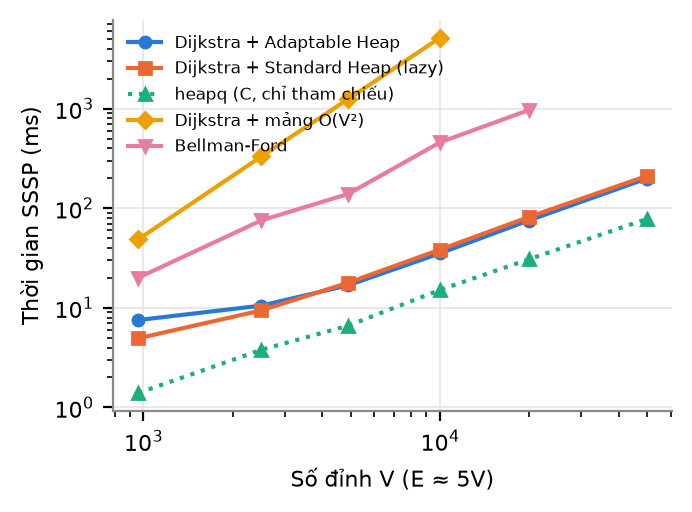
\includegraphics[width=\columnwidth]{sssp_time}
\caption{Thời gian SSSP trên đồ thị dạng mạng đường ($E\approx 5V$, thang log--log).}
\label{fig:sssp-time}
\end{figure}

\begin{figure*}[t]
\centering
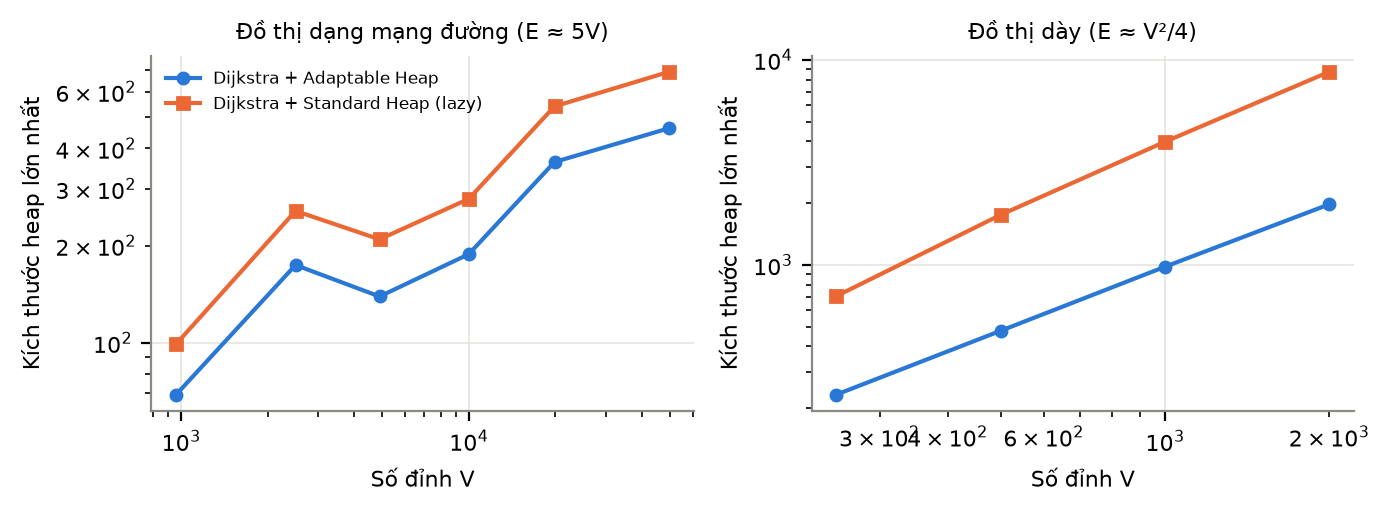
\includegraphics[width=0.49\textwidth]{heap_peak}\hfill
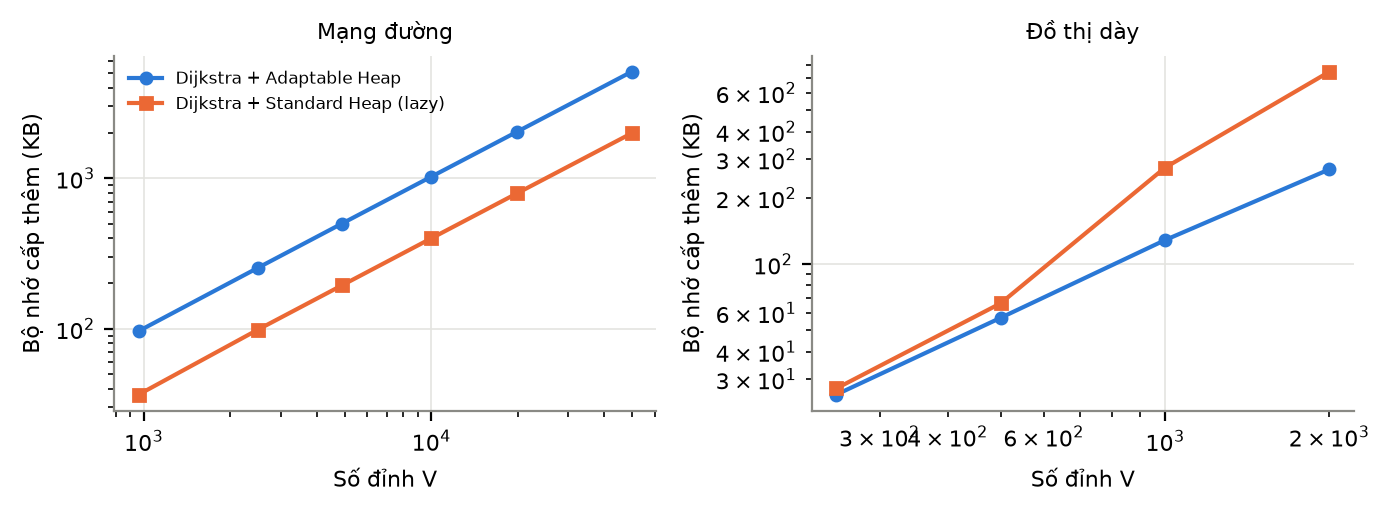
\includegraphics[width=0.49\textwidth]{sssp_memory}
\caption{Trái: kích thước heap lớn nhất. Phải: bộ nhớ cấp thêm. Ở mỗi hình, panel trái là đồ thị dạng mạng đường,
panel phải là đồ thị dày.}
\label{fig:heap}
\end{figure*}

Bảng~\ref{tab:sssp-osm} và Hình~\ref{fig:sssp-time} cho ba nhận xét.

\textbf{(i) Trên mạng đường, lazy heap không phình to.} Về lý thuyết, lazy heap có thể chứa tới $E$ phần tử. Thực tế, ở
$V=49\,729$ heap lớn nhất chỉ có 691 phần tử, còn heap của Adaptable Heap có 462 phần tử, tức dưới 1{,}5\% số đỉnh
(Hình~\ref{fig:heap}). Lý do: đồ thị đường bộ gần phẳng và bậc nhỏ, nên tập đỉnh đang chờ của Dijkstra chỉ là một "mặt sóng"
mỏng quanh nguồn. Khi số phần tử trùng lặp ít, lợi thế cận $O(V)$ của Adaptable Heap không thể hiện ra. Ngược lại, mỗi đỉnh
được chạm tới đều cần một đối tượng Locator, nên Adaptable Heap tốn bộ nhớ gấp khoảng 2{,}5 lần (5\,099 KB so với 1\,989 KB)
và chậm hơn 5--20\%. Hai đường thời gian gần như trùng nhau và cùng tăng tuyến tính theo $V$ trên thang log, khớp với cận
$O((V+E)\log V)$.

\textbf{(ii) Trên đồ thị dày, Adaptable Heap thắng.} Mỗi đỉnh có $V/4$ cạnh vào, nên decrease-key xảy ra liên tục. Ở
$V=2000$ ($E\approx 10^6$), lazy heap đạt 8\,737 phần tử so với 1\,974 của Adaptable Heap (gấp 4{,}4 lần) và dùng
747 KB so với 269 KB. Adaptable Heap nhanh hơn 16\% (123{,}6 ms so với 146{,}6 ms). Như vậy lợi ích của Locator phụ thuộc vào
\emph{tỉ lệ decrease-key trên số đỉnh}, không phải lúc nào cũng có.

\textbf{(iii) Baseline.} Dijkstra dùng mảng $O(V^2)$ chậm hơn 146 lần ở $V=10\,000$ (5{,}14 s so với 35 ms) và quá
120~s trên bản đồ thật. Kể cả trên đồ thị dày, nơi $O(V^2)$ về lý thuyết là tối ưu, bản mảng vẫn chậm gấp 2{,}8 lần, vì vòng
quét $V$ phần tử chạy hoàn toàn trong trình thông dịch. Bellman-Ford dừng sớm chậm hơn 13 lần ở $V=10\,000$ và 26 lần trên
bản đồ thật. Nó không bị chậm tới mức $O(VE)$ đầy đủ vì số vòng lặp chỉ bằng số cạnh của đường đi ngắn nhất dài nhất.
\texttt{heapq} nhanh hơn heap Python của nhóm 2{,}6--3{,}2 lần ở mọi kích thước. Đây là hằng số của mã C, còn độ dốc của hai
đường như nhau.

\textbf{Reroute.} Trên bản đồ thật, một Traffic Incident nằm ngoài tuyến được bỏ qua sau 0{,}4 ms (chỉ kiểm tra mặt nạ
\texttt{on\_route}). Một sự cố trên tuyến buộc phải chạy lại Dijkstra từ vị trí xe, mất khoảng 100--110 ms. Đây là số đo từ
một lần thao tác trên giao diện demo, chưa phải trung vị nhiều lần, nhưng chênh lệch hơn hai bậc là đúng như phân tích
$O(L)$ so với $O((V+E)\log V)$.

\begin{figure}[t]
\centering
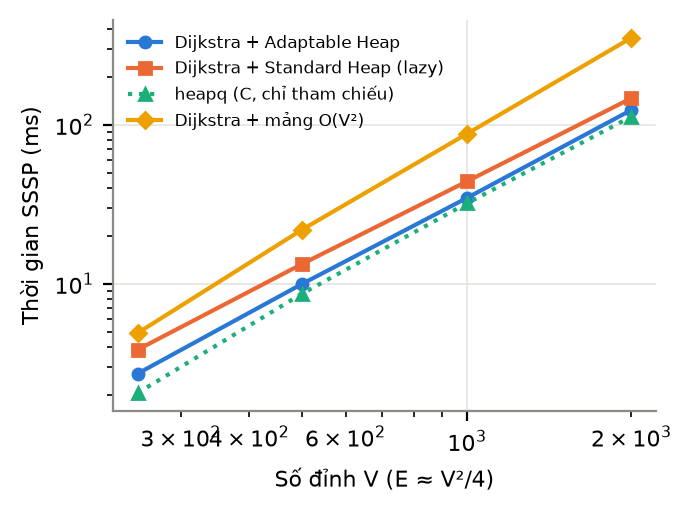
\includegraphics[width=\columnwidth]{sssp_dense_time}
\caption{SSSP trên đồ thị dày ($E\approx V^2/4$).}
\label{fig:dense}
\end{figure}

\subsection{Union-Find}

\begin{figure*}[t]
\centering
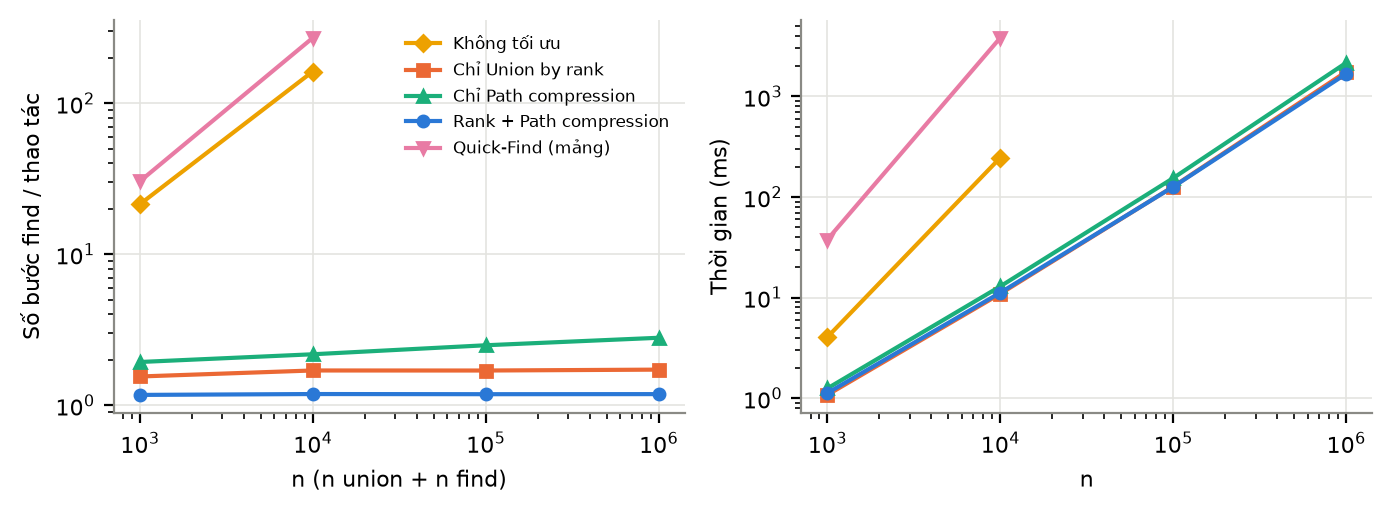
\includegraphics[width=0.49\textwidth]{dsu}\hfill
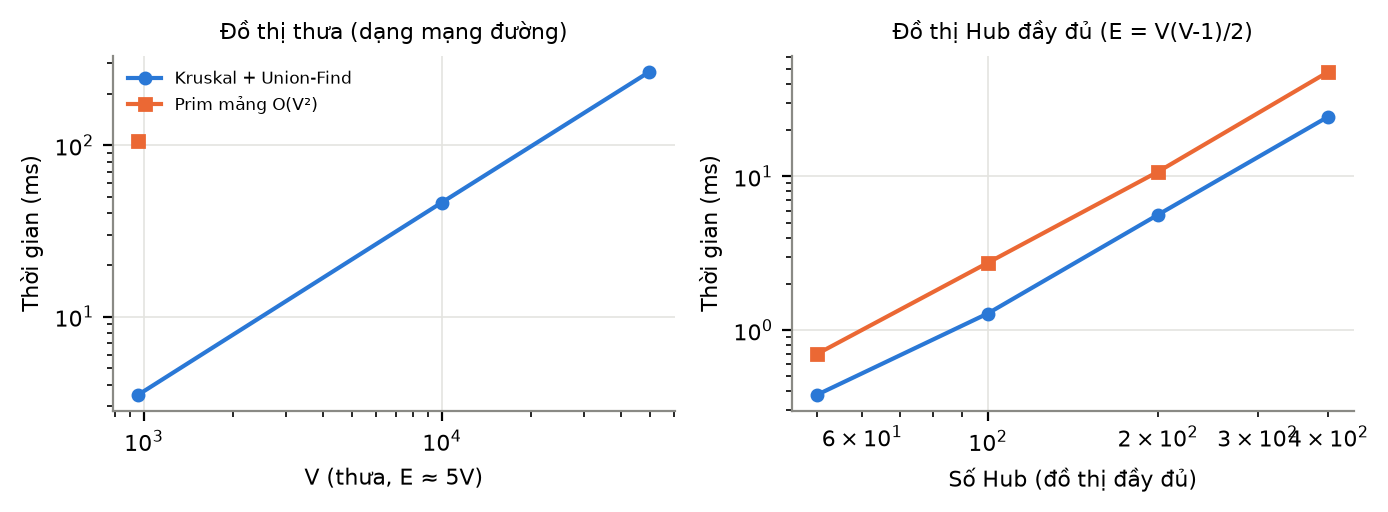
\includegraphics[width=0.49\textwidth]{mst}
\caption{Trái: Union-Find với $n$ phép union và $n$ phép find ngẫu nhiên (số bước trên một thao tác; thời gian).
Phải: thời gian tìm MST trên đồ thị thưa và đồ thị Hub đầy đủ.}
\label{fig:dsu-mst}
\end{figure*}

\begin{table}[t]
\centering
\caption{Số bước duyệt con trỏ \texttt{parent} trung bình trên một thao tác}
\label{tab:dsu}
\begin{tabular}{lrrrr}
\toprule
Biến thể & $n=10^3$ & $10^4$ & $10^5$ & $10^6$ \\
\midrule
Rank + Path compression & 1{,}17 & 1{,}19 & 1{,}18 & 1{,}19 \\
Chỉ Union by rank & 1{,}55 & 1{,}70 & 1{,}70 & 1{,}72 \\
Chỉ Path compression & 1{,}93 & 2{,}18 & 2{,}50 & 2{,}80 \\
Không tối ưu & 21{,}4 & 162 & timeout & -- \\
Quick-Find (số lần ghi) & 30{,}4 & 271 & -- & -- \\
\bottomrule
\end{tabular}
\end{table}

Bảng~\ref{tab:dsu} là minh chứng thực nghiệm cho cận khấu hao $O(\alpha(n))$. Khi bật cả hai tối ưu, số bước trên một thao
tác giữ ở 1{,}17--1{,}19 trong khi $n$ tăng 1000 lần. Thời gian tăng tuyến tính theo số thao tác: 1{,}68 s cho $2\cdot 10^6$
thao tác, tức khoảng 0{,}84~$\mu$s mỗi thao tác. Chỉ dùng path compression thì số bước tăng chậm, đúng với cận
$O(\log n)$ khấu hao. Chỉ dùng union by rank thì số bước ổn định ở mức cao hơn, vì chiều cao cây bị chặn bởi $\log_2 n$ nhưng
không giảm đi. Bản không tối ưu tăng gần tuyến tính và quá thời gian ở $n=10^5$. Quick-Find tốn 3{,}8 s ở $n=10^4$, chậm hơn
bản tối ưu 340 lần, vì mỗi phép union phải gán lại nhãn cho tới $n$ phần tử.

\subsection{Cây khung nhỏ nhất}

Kruskal và Prim luôn cho cùng tổng trọng số, đây cũng là cách kiểm tra chéo tính đúng. Trên đồ thị thưa, Kruskal xử lý
49\,729 đỉnh và 248\,645 cạnh trong 268 ms. Prim mảng cần ma trận $V\times V$, mất 105 ms ngay ở $V=961$ và quá thời gian
ở $V=10\,000$. Trên đồ thị Hub đầy đủ, ta dự đoán Prim $O(V^2)$ sẽ thắng Kruskal $O(V^2\log V)$, nhưng số đo cho thấy
\emph{Kruskal vẫn nhanh hơn khoảng 2 lần} (24{,}5 ms so với 48{,}0 ms ở 400 Hub). Nguyên nhân: bước sắp xếp
$O(E\log E)$ của Kruskal dùng \texttt{list.sort} viết bằng C, còn vòng $O(V^2)$ của Prim là Python thuần. Ở quy mô vài trăm
Hub, hệ số $\log V\approx 9$ nhỏ hơn chênh lệch hằng số giữa C và Python. Đây là một ví dụ cho thấy cận tiệm cận chỉ dự đoán
xu hướng khi $n$ đủ lớn, không dự đoán thứ hạng ở một kích thước cụ thể. Trong demo, Backbone giữa 24 Hub mất 3{,}8 s, gần
như toàn bộ là 24 lần Dijkstra để dựng ma trận; riêng phần MST không đáng kể.

\subsection{Xếp hàng lên xe và thứ tự giao}

\begin{figure}[t]
\centering
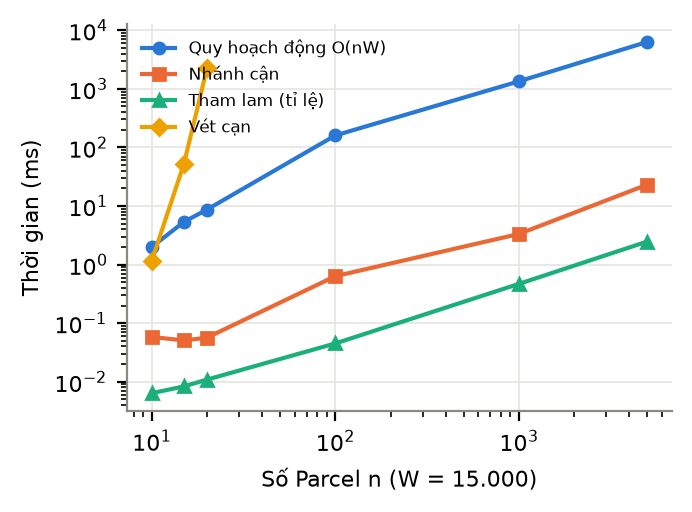
\includegraphics[width=\columnwidth]{knapsack}
\caption{Thời gian giải 0/1 Knapsack, $W=15\,000$ (xe 1{,}5 tấn).}
\label{fig:knapsack}
\end{figure}

\textbf{Knapsack} (Hình~\ref{fig:knapsack}). Khi $W$ cố định, thời gian quy hoạch động tăng tuyến tính theo $n$: 160 ms,
1{,}34 s và 6{,}33 s với $n=100$, 1000 và 5000. Bảng truy vết chiếm 2 MB, 15 MB và 74 MB, khớp với $n(W+1)$ byte. Vét cạn
tăng gấp đôi khi thêm mỗi Parcel và mất 2{,}2 s ở $n=20$. Nhánh cận chỉ mất 3{,}3 ms ở $n=1000$ và 23 ms ở $n=5000$, nhanh
hơn quy hoạch động tới 270 lần. Kết quả này chỉ đúng cho dữ liệu ngẫu nhiên, khi khối lượng và cước độc lập nhau, nên cận
phân số cắt nhánh rất sớm. Trường hợp xấu nhất của nhánh cận vẫn là hàm mũ, và nhóm chưa thử bộ dữ liệu có khối lượng và cước
tương quan chặt (trường hợp khó cho nhánh cận). Tham lam theo tỉ lệ thiếu 5{,}9\% so với tối ưu ở $n=10$, nhưng chỉ còn
0{,}05\% ở $n=5000$: khi có nhiều Parcel nhỏ so với $W$, phần dư cuối cùng không đáng kể.

\begin{figure}[t]
\centering
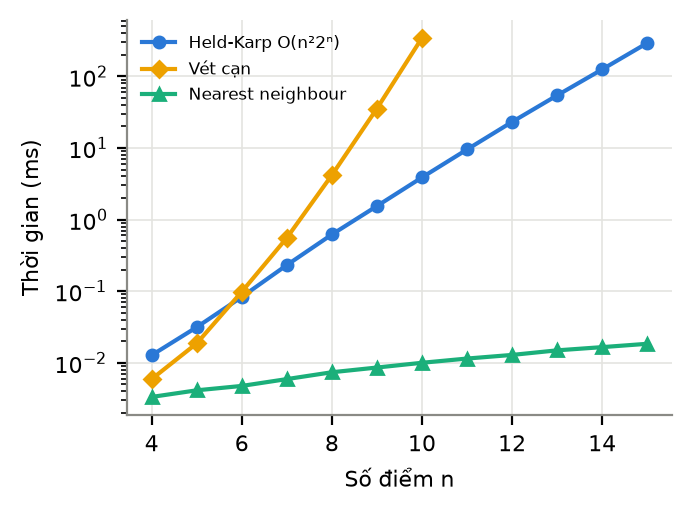
\includegraphics[width=\columnwidth]{tsp}
\caption{Thời gian TSP bất đối xứng (thang log): Held-Karp, vét cạn, nearest neighbour.}
\label{fig:tsp}
\end{figure}

\textbf{TSP} (Hình~\ref{fig:tsp}). Held-Karp tăng khoảng 2{,}3 lần mỗi khi thêm một điểm và mất 293 ms ở $n=15$. Vét cạn tăng
khoảng $n$ lần mỗi bước và đã mất 345 ms ở $n=10$. Ở cùng $n=10$, Held-Karp nhanh hơn 89 lần (3{,}9 ms). Nearest neighbour gần
như tức thời nhưng dài hơn tối ưu 5--41\% (trung bình 21\%). Với một chuyến giao, chênh lệch đó tương đương vài chục phút chạy
xe. Vì vậy giới hạn 12 điểm mỗi chuyến (khoảng 23 ms) là điểm cân bằng hợp lý giữa tối ưu và thời gian phản hồi.

\subsection{Giới hạn của thực nghiệm}

(1) Mọi cài đặt viết bằng Python, nên hằng số của trình thông dịch có thể làm đảo thứ hạng so với lý thuyết, như đã thấy ở
Prim và Kruskal. (2) Chỉ đo trên một máy. (3) \texttt{tracemalloc} chỉ đếm bộ nhớ do Python cấp phát, không đếm bộ nhớ của
tiến trình. (4) Đỉnh của bản đồ thật gồm cả điểm uốn của đường, nên số đỉnh lớn hơn số giao lộ thật. (5) Vận tốc là giả định
theo loại đường, chưa có dữ liệu giao thông thực tế. (6) Thời gian reroute là số đo trên demo, chưa lặp lại nhiều lần.

\section{Kết luận}

Nhóm đã xây dựng một hệ thống hoàn chỉnh cho Đề tài 4: từ dữ liệu bản đồ thật, qua các cấu trúc dữ liệu tự cài đặt, tới giao
diện demo cho phép tìm tuyến, gây sự cố giao thông, xem mạng xương sống giữa các kho, phân cụm đơn hàng và lập chuyến xe.
Lõi giải thuật khoảng 1\,300 dòng Python không dùng \texttt{dict}, \texttt{set} hay \texttt{heapq}, và quy tắc này được một
test phân tích cú pháp kiểm tra tự động. Mỗi giải thuật có test đối chiếu với lời giải chuẩn: Dijkstra với Bellman-Ford,
Kruskal với Prim, Knapsack và Held-Karp với vét cạn, Union-Find với BFS.

Kết quả thực nghiệm khớp với phân tích Big-O ở những chỗ mà lý thuyết dự đoán xu hướng: cận $O(\alpha(n))$ của Union-Find,
độ tăng $O(n^2 2^n)$ so với $O(n!)$ của TSP, tính tuyến tính theo $n$ của Knapsack khi $W$ cố định. Thực nghiệm cũng chỉ ra hai
chỗ cần đọc lý thuyết cẩn thận hơn. Thứ nhất, lợi thế của Adaptable Priority Queue phụ thuộc vào tỉ lệ decrease-key, vốn rất
thấp trên mạng đường. Thứ hai, ở quy mô vừa phải, hằng số của trình thông dịch có thể làm đảo thứ hạng giữa hai giải thuật có
cận khác nhau, như trường hợp Prim và Kruskal.

\textbf{Hướng phát triển.} Dùng A* với heuristic khoảng cách đường chim bay và Dijkstra hai chiều để giảm số đỉnh phải duyệt;
cập nhật đường đi ngắn nhất tăng dần thay vì tính lại; rút gọn các đỉnh bậc 2 của dữ liệu OSM; mở rộng bài toán lập chuyến
thành VRP nhiều xe có khung giờ giao; cài lại phần lõi bằng C++ để so sánh các giải thuật mà không bị ảnh hưởng bởi hằng số
của trình thông dịch.


\bibliographystyle{IEEEtran}
\bibliography{refs}

\end{document}
